\documentclass{article}
\usepackage{graphicx}
\usepackage{float}
\graphicspath{{Illustrations/}}

\title{\textbf{COMP1044 Coursework Assignment 2 Report B} \\ Group 15 / Chew Language}
\author{
	Leong Chang Yung, 20307078
	\and
	Lucas Dylan Purnell, 20197316
	\and
	Tan Zhun Xian, 20313854
	\and
	Chong Hao Wei, 20194465
	\and
	Morhaf Allababidi, 20195867
	\and
	Thomas Tan Kean Yew, 20316601
}
\date{\today}

\begin{document}
\maketitle
\newpage

\section{Entity Relation Diagram}
	\begin{figure}[h!]
		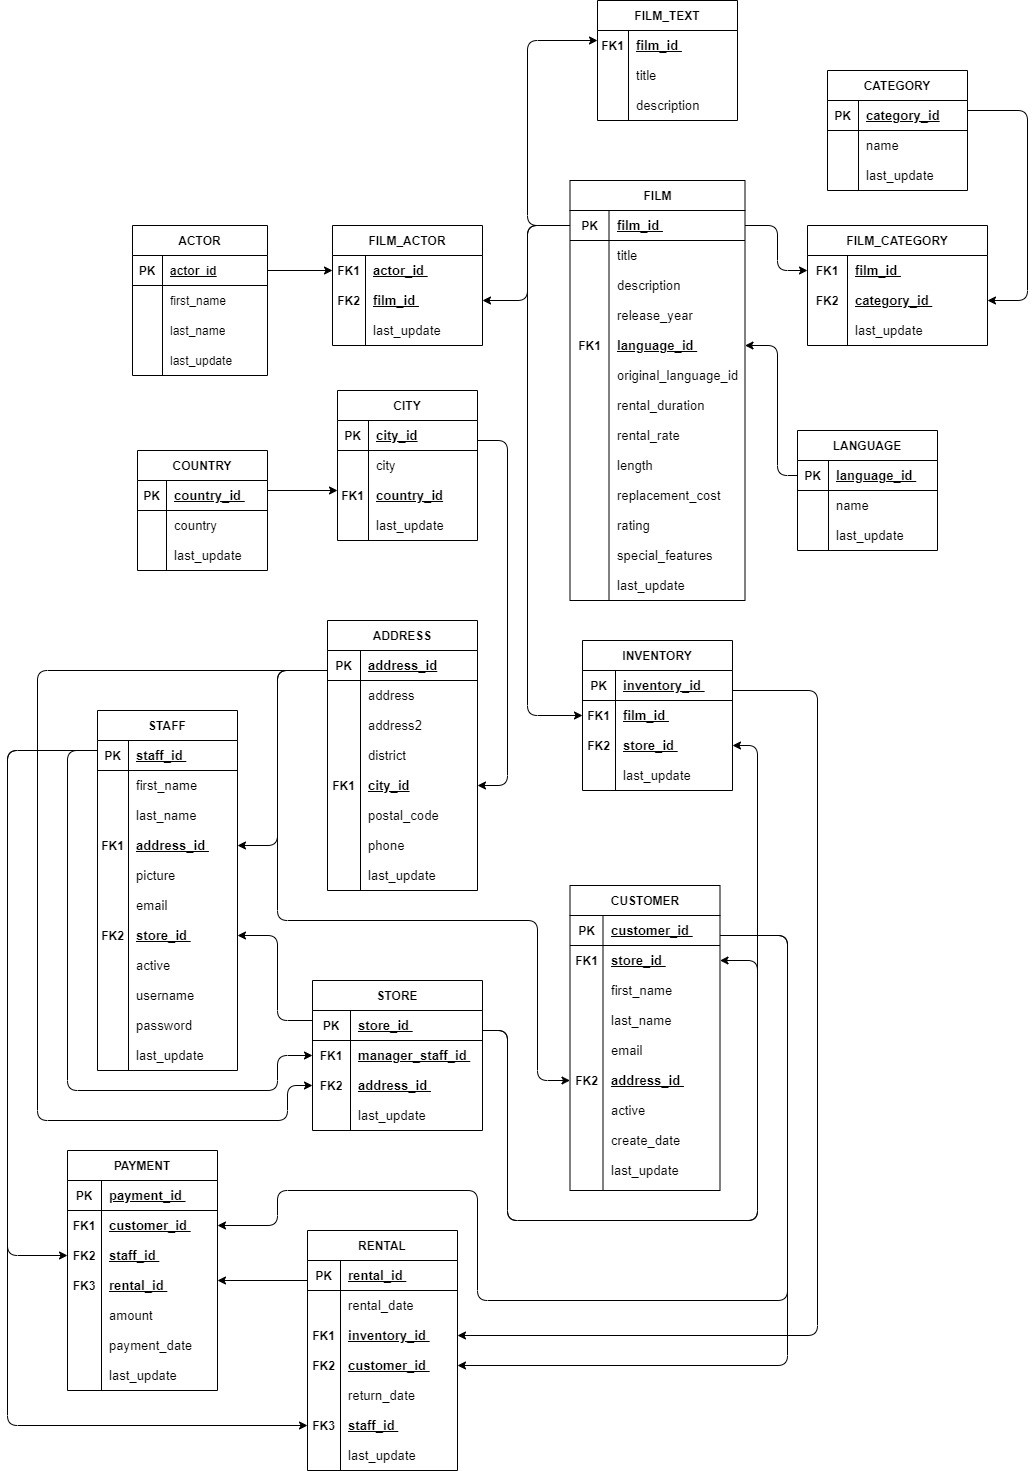
\includegraphics[height=.8\textheight, width=\textwidth]{er_diagram}
		\caption{Proposed Entity Relation Diagram arrangement. \protect\footnotemark}	
	\end{figure}
	\footnotetext{This diagram is based on available table data provided.}


\section{Database Creation}
	\begin{figure}[H]
		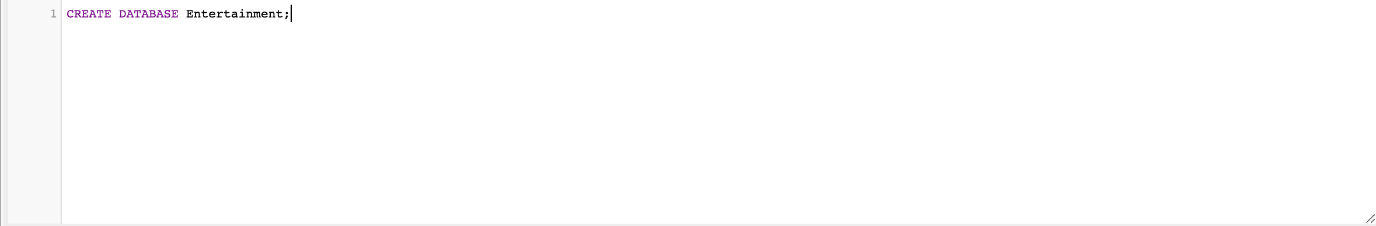
\includegraphics[width=\textwidth]{database_create}
		\caption{Creation of database "Entertainment"}	
	\end{figure}
	\rule{\textwidth}{0.4pt}
\section{Creation and Insertion of Tables}
	\begin{figure}[H]
		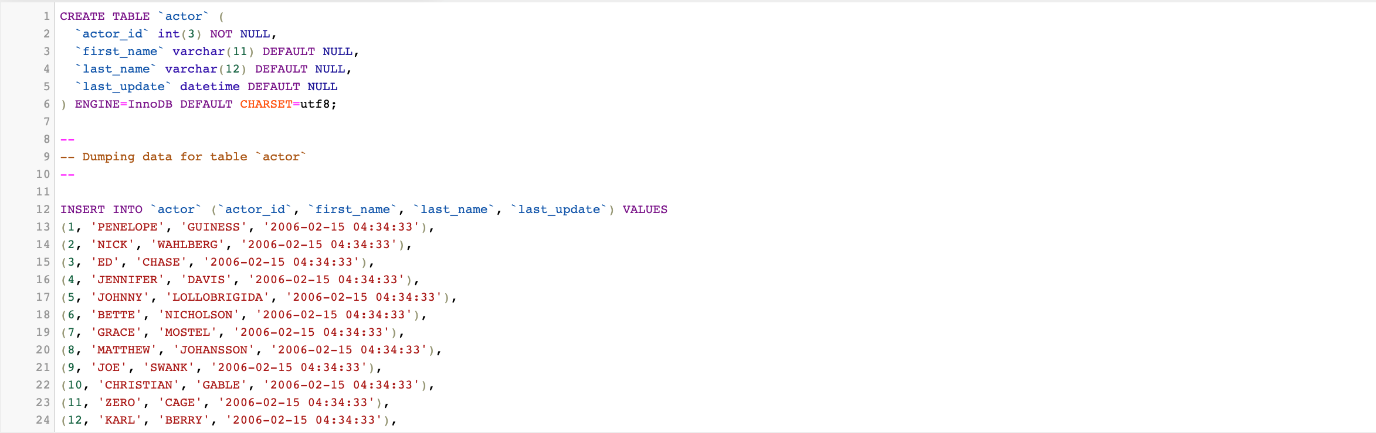
\includegraphics[width=\textwidth]{table_actor_cins}
		\caption{Creation and Insertion of table "Actor"}	
	\end{figure}
	\begin{figure}[H]
		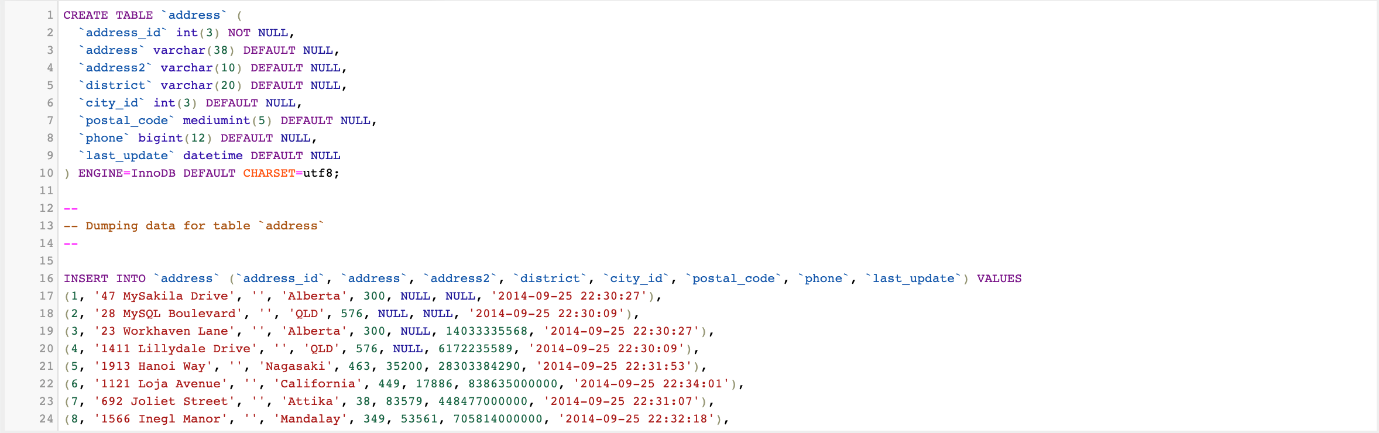
\includegraphics[width=\textwidth]{table_address_cins}
		\caption{Creation and Insertion of table "Address"}	
	\end{figure}
	\begin{figure}[H]
		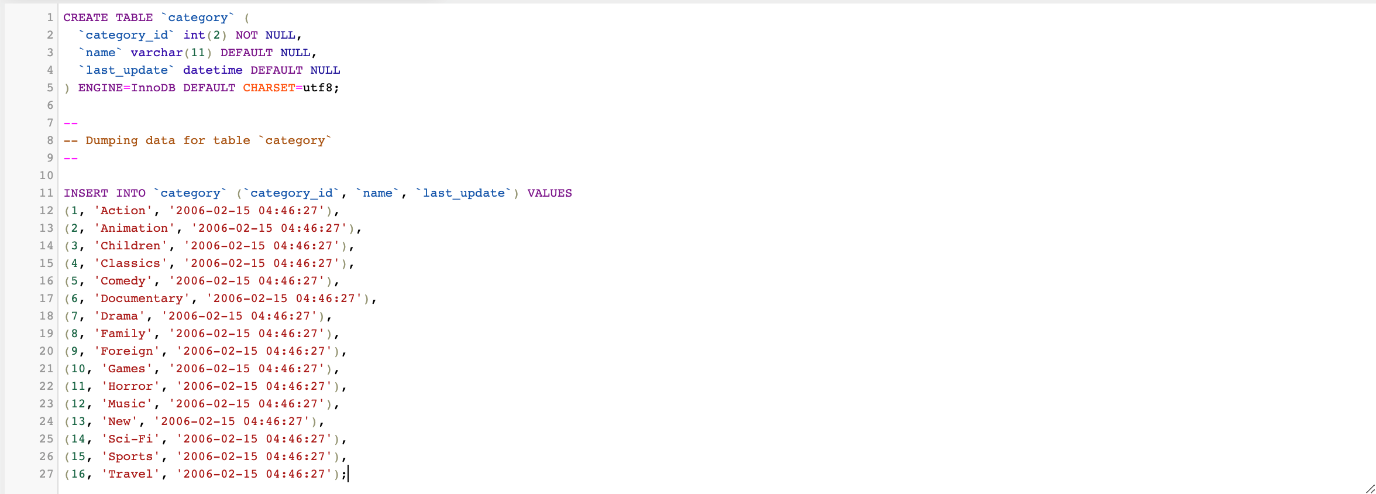
\includegraphics[width=\textwidth]{table_category_cins}
		\caption{Creation and Insertion of table "Category"}	
	\end{figure}
	\begin{figure}[H]
		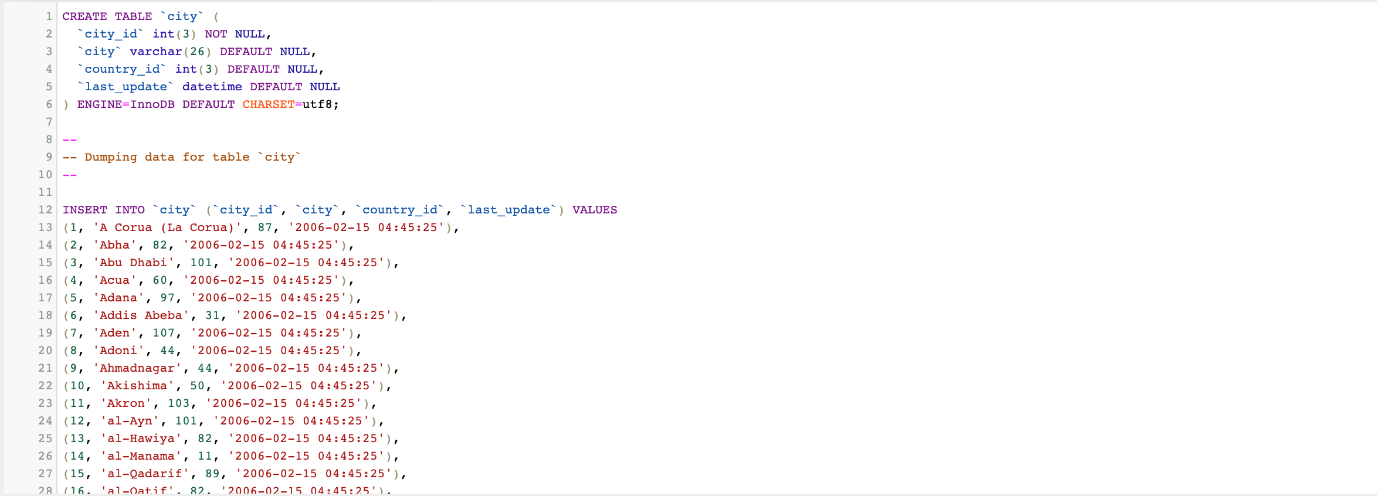
\includegraphics[width=\textwidth]{table_city_cins}
		\caption{Creation and Insertion of table "City"}	
	\end{figure}
	\begin{figure}[H]
		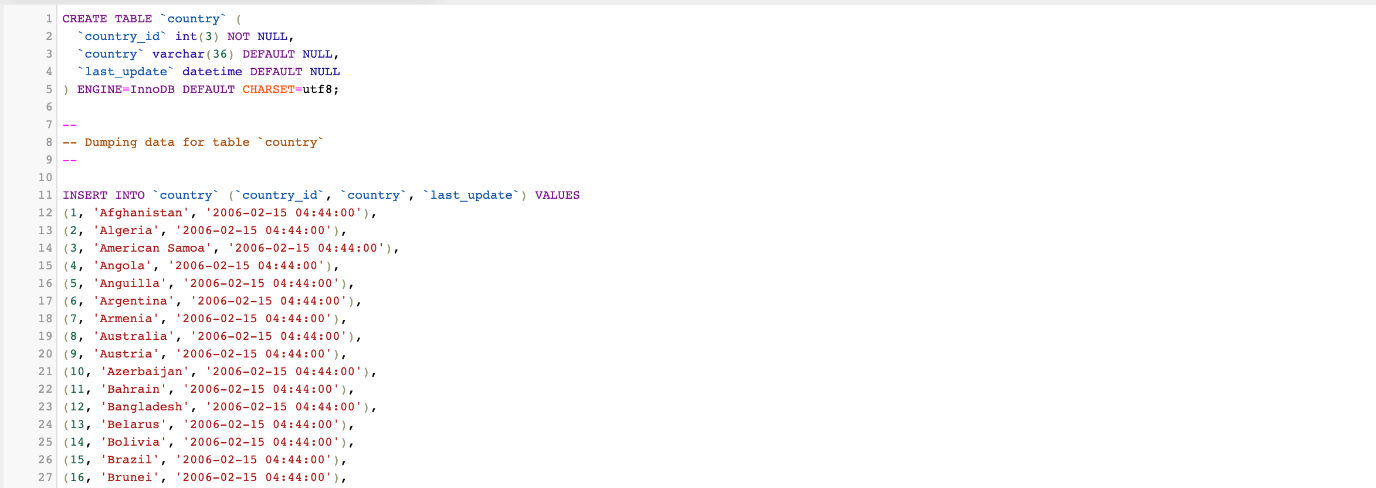
\includegraphics[width=\textwidth]{table_country_cins}
		\caption{Creation and Insertion of table "Country"}	
	\end{figure}
	\begin{figure}[H]
		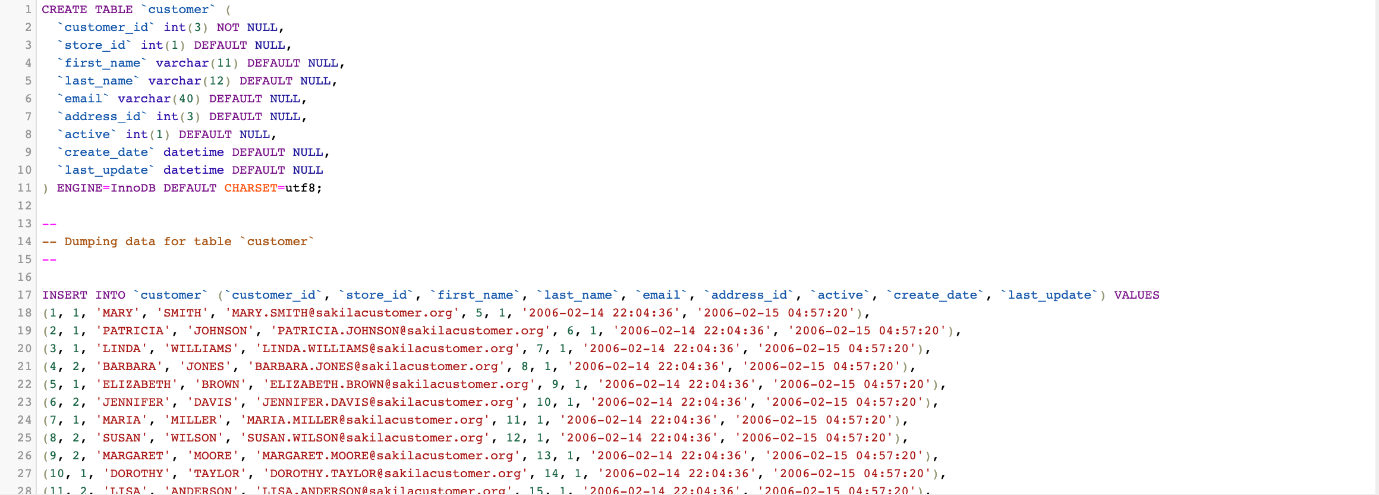
\includegraphics[width=\textwidth]{table_customer_cins}
		\caption{Creation and Insertion of table "Customer"}	
	\end{figure}
	\begin{figure}[H]
		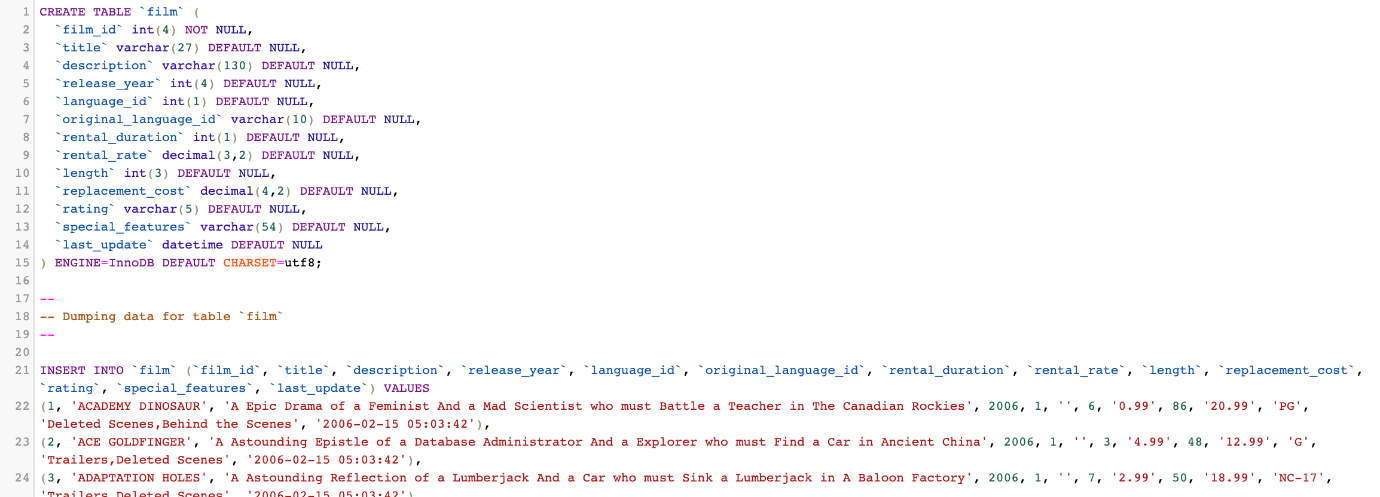
\includegraphics[width=\textwidth]{table_film_cins}
		\caption{Creation and Insertion of table "Film"}	
	\end{figure}
	\begin{figure}[H]
		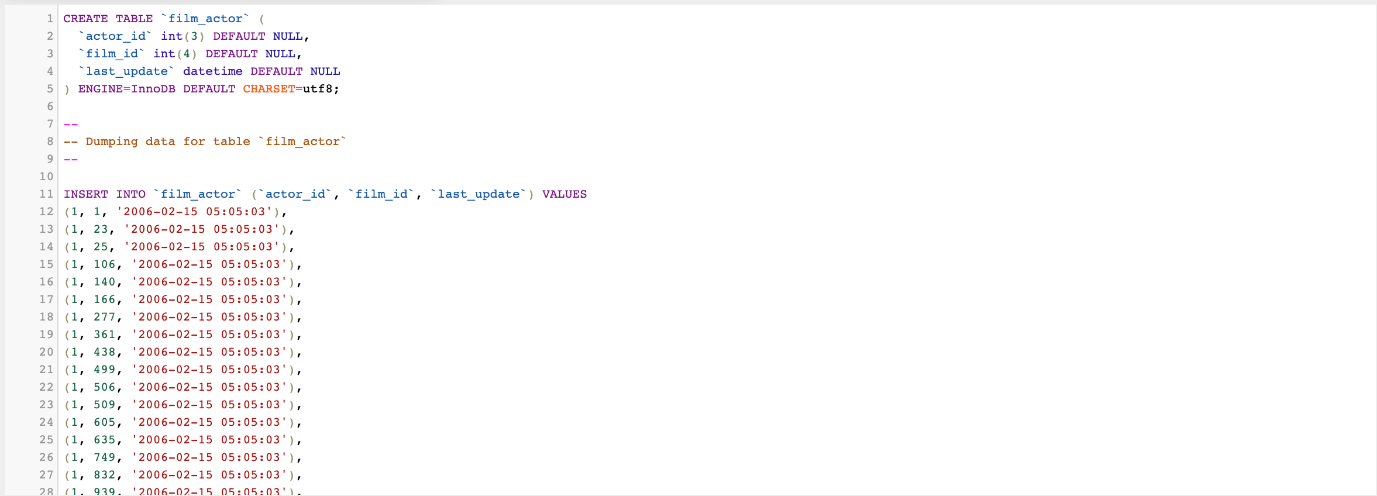
\includegraphics[width=\textwidth]{table_filmactor_cins}
		\caption{Creation and Insertion of table "Film\textunderscore Actor"}	
	\end{figure}
	\begin{figure}[H]
		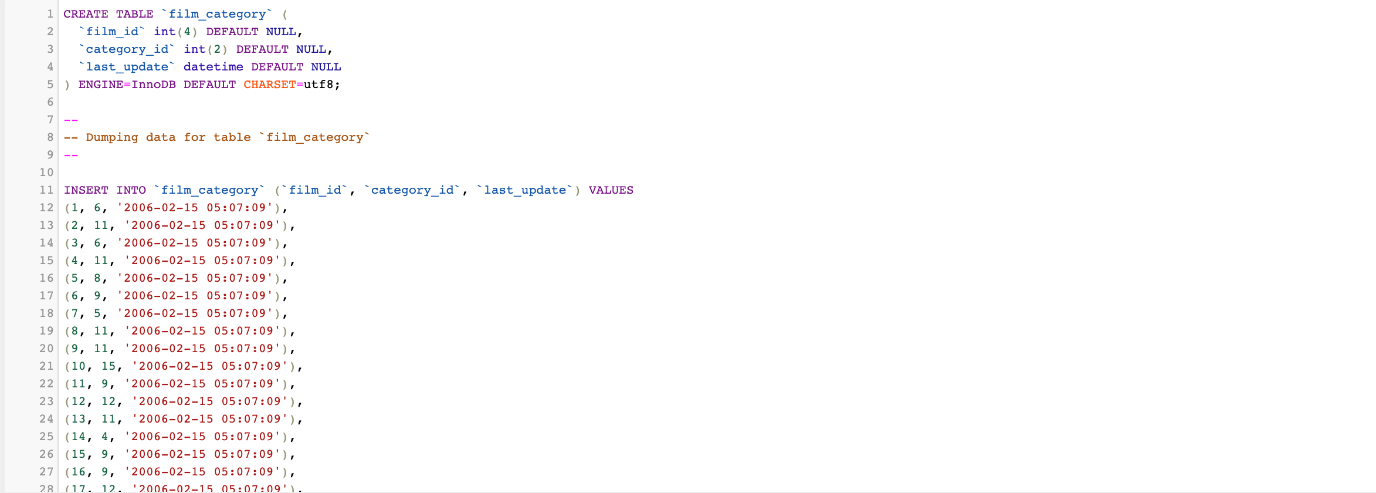
\includegraphics[width=\textwidth]{table_filmcategory_cins}
		\caption{Creation and Insertion of table "Film\textunderscore Category"}	
	\end{figure}
	\begin{figure}[H]
		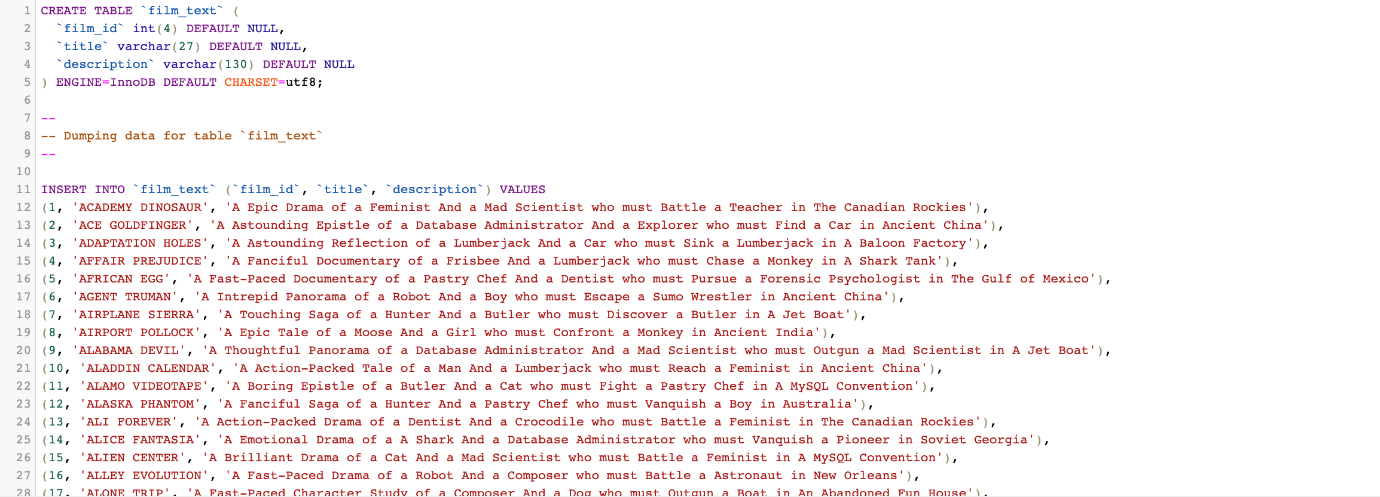
\includegraphics[width=\textwidth]{table_filmtext_cins}
		\caption{Creation and Insertion of table "Film\textunderscore Text"}	
	\end{figure}
	\begin{figure}[H]
		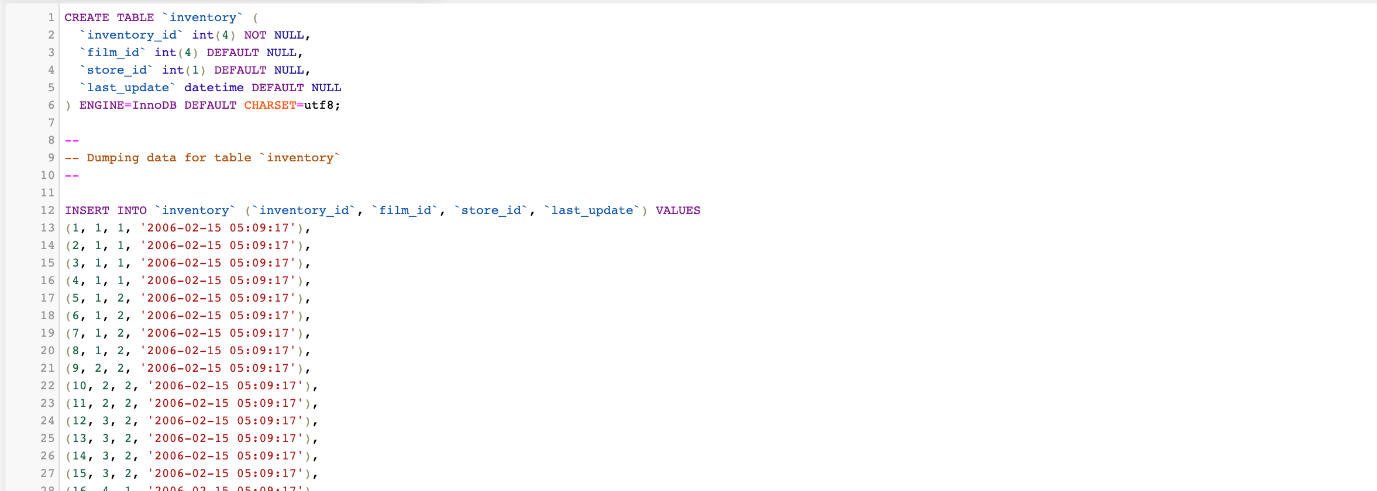
\includegraphics[width=\textwidth]{table_inventory_cins}
		\caption{Creation and Insertion of table "Inventory"}	
	\end{figure}
	\begin{figure}[H]
		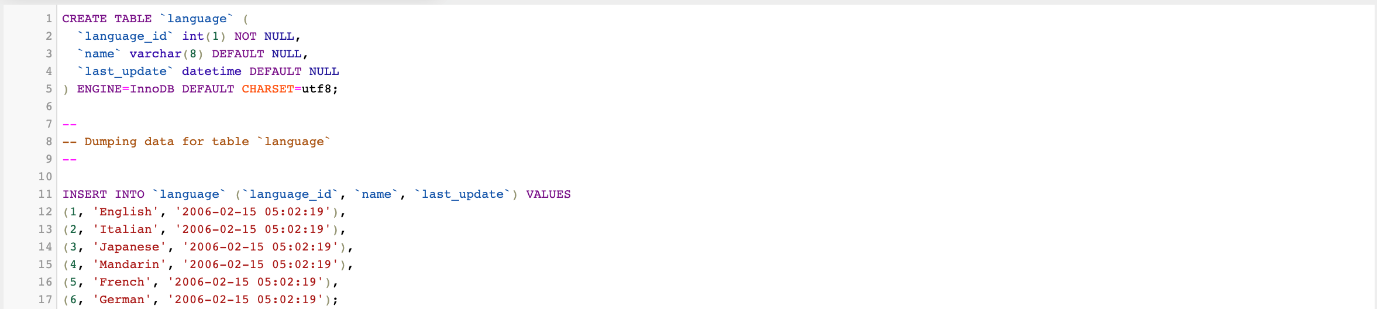
\includegraphics[width=\textwidth]{table_language_cins}
		\caption{Creation and Insertion of table "Language"}	
	\end{figure}
	\begin{figure}[H]
		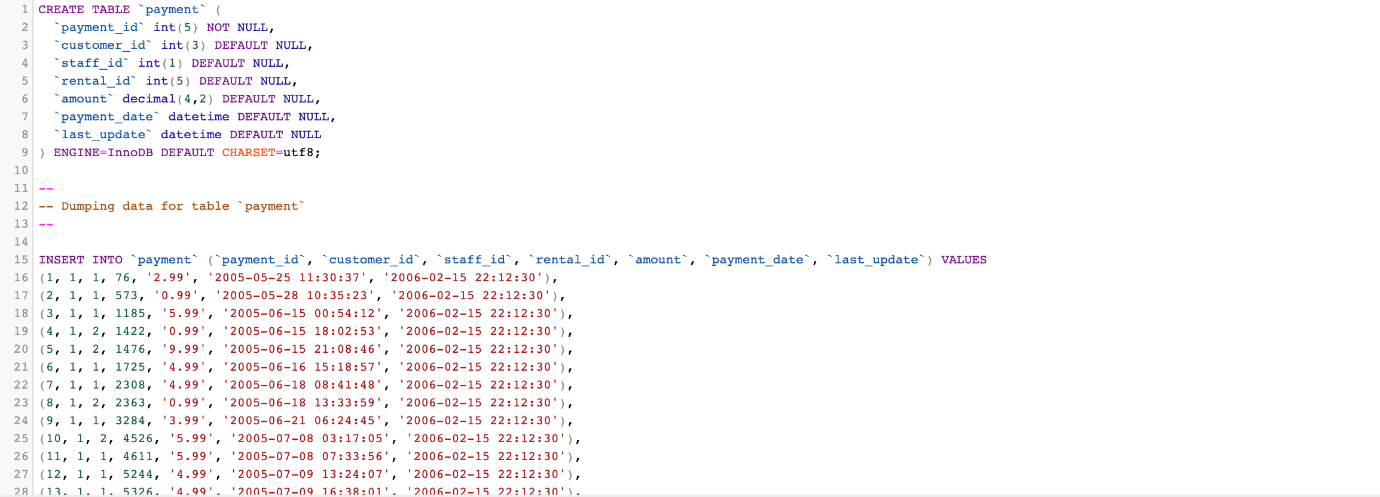
\includegraphics[width=\textwidth]{table_payment_cins}
		\caption{Creation and Insertion of table "Payment"}	
	\end{figure}
	\begin{figure}[H]
		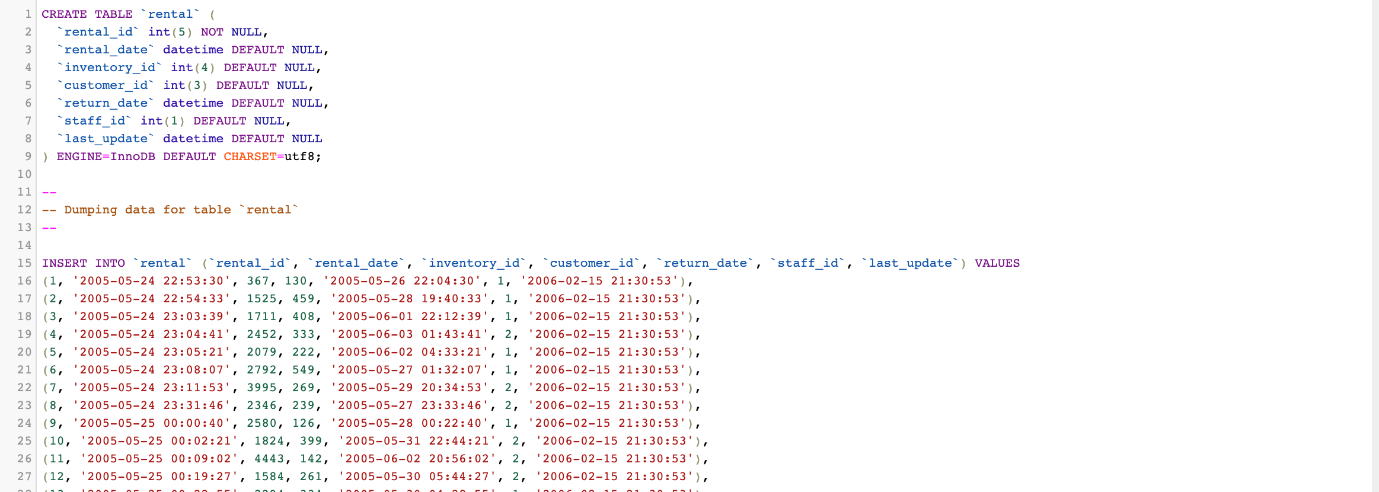
\includegraphics[width=\textwidth]{table_rental_cins}
		\caption{Creation and Insertion of table "Rental"}	
	\end{figure}
	\begin{figure}[H]
		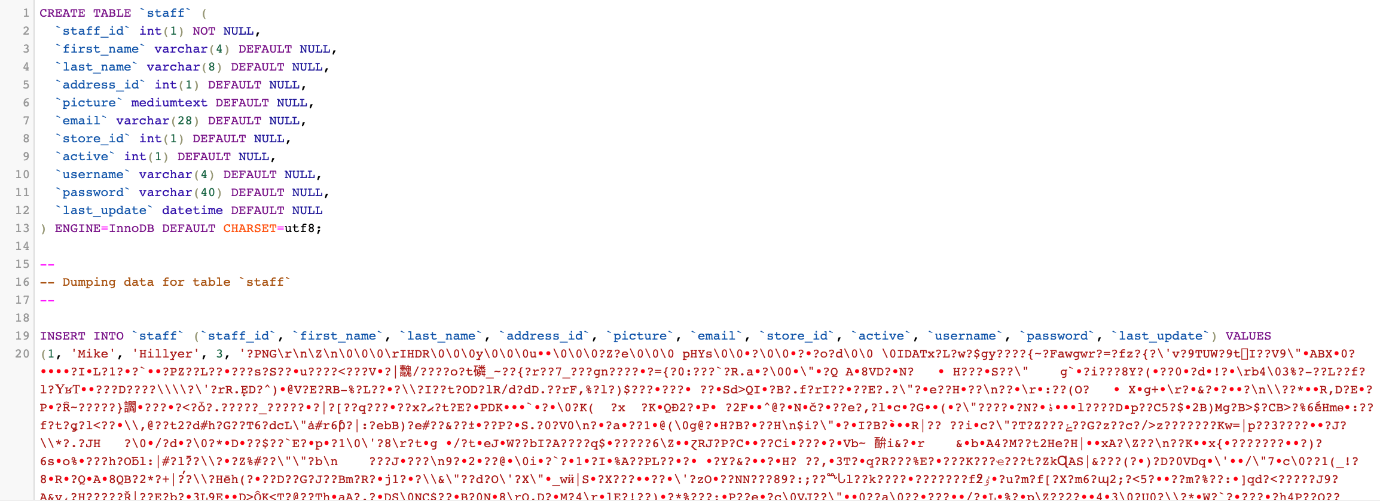
\includegraphics[width=\textwidth]{table_staff_cins}
		\caption{Creation and Insertion of table "Staff"}	
	\end{figure}
	\begin{figure}[H]
		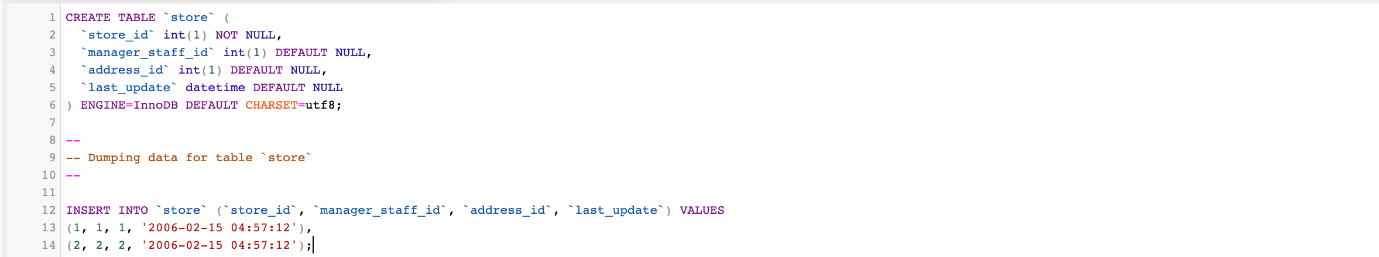
\includegraphics[width=\textwidth]{table_store_cins}
		\caption{Creation and Insertion of table "Store"}	
	\end{figure}

\section{Table Constraints (Foreign Keys)}
	\begin{figure}[H]
		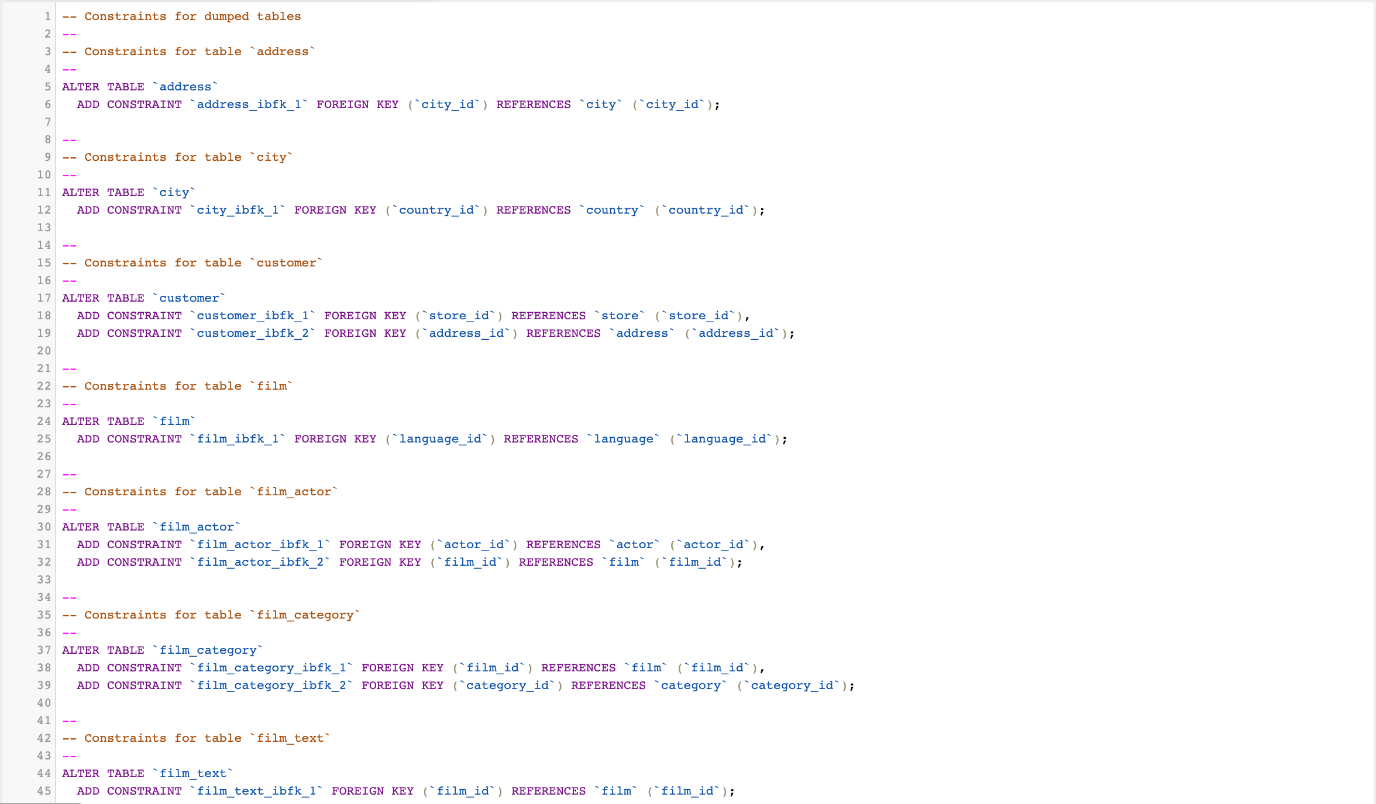
\includegraphics[width=\textwidth]{tableconstraints1}
		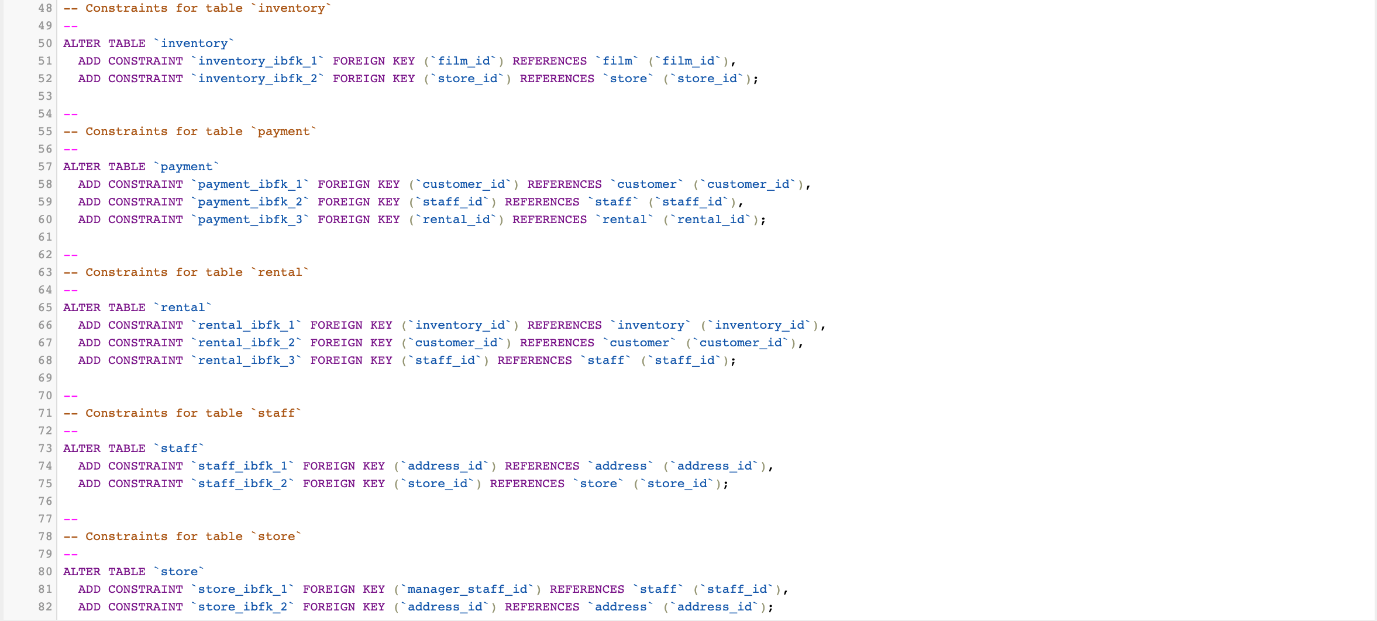
\includegraphics[width=\textwidth]{tableconstraints2}
	\end{figure}

\section{Table Indexes (Primary/Foreign Keys)}
	\begin{figure}[H]
		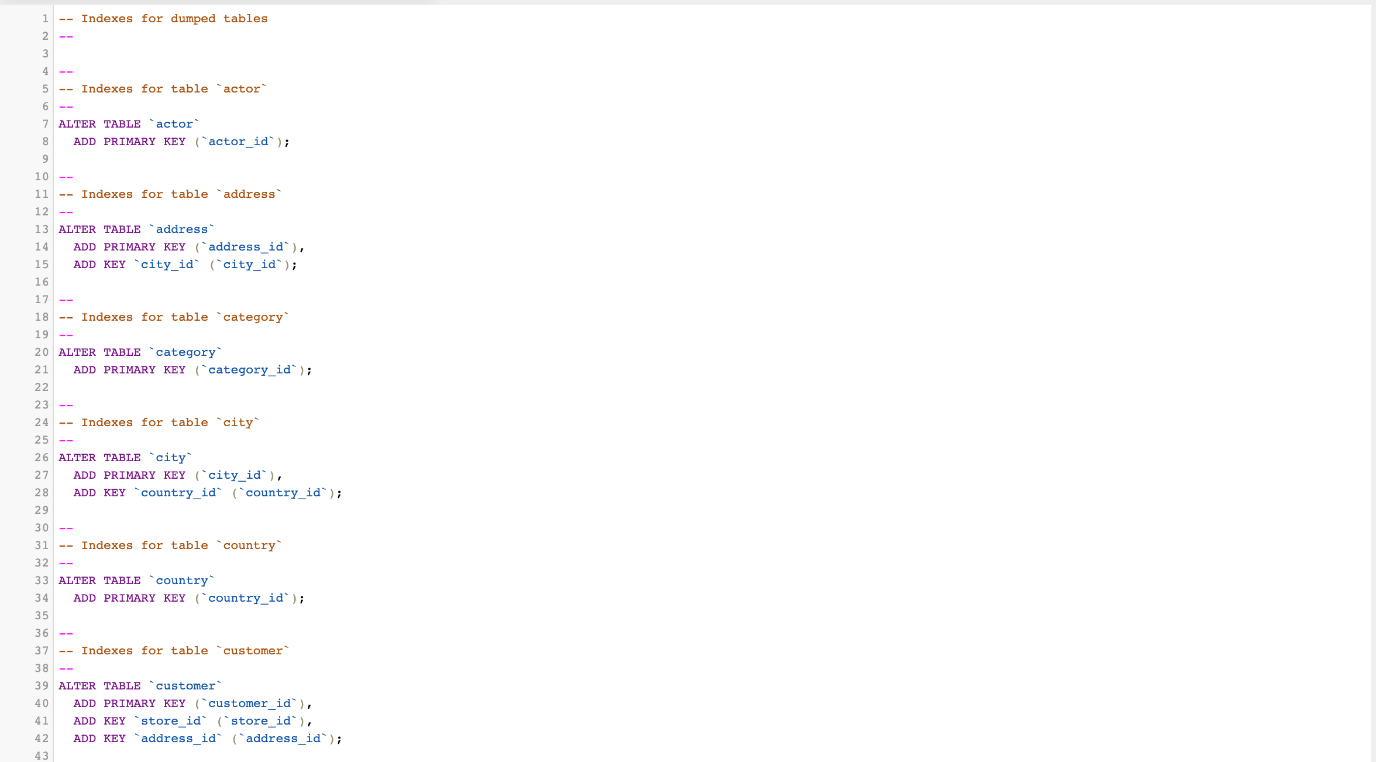
\includegraphics[width=\textwidth]{tableindexkeys1}
		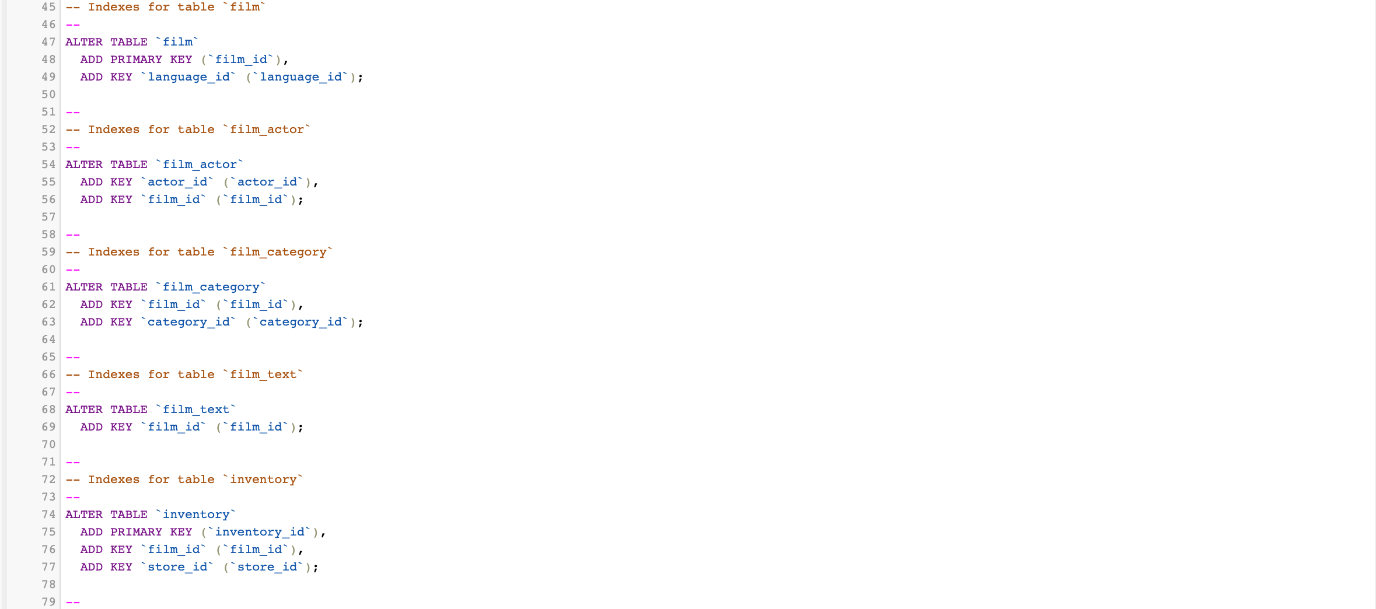
\includegraphics[width=\textwidth]{tableindexkeys2}
		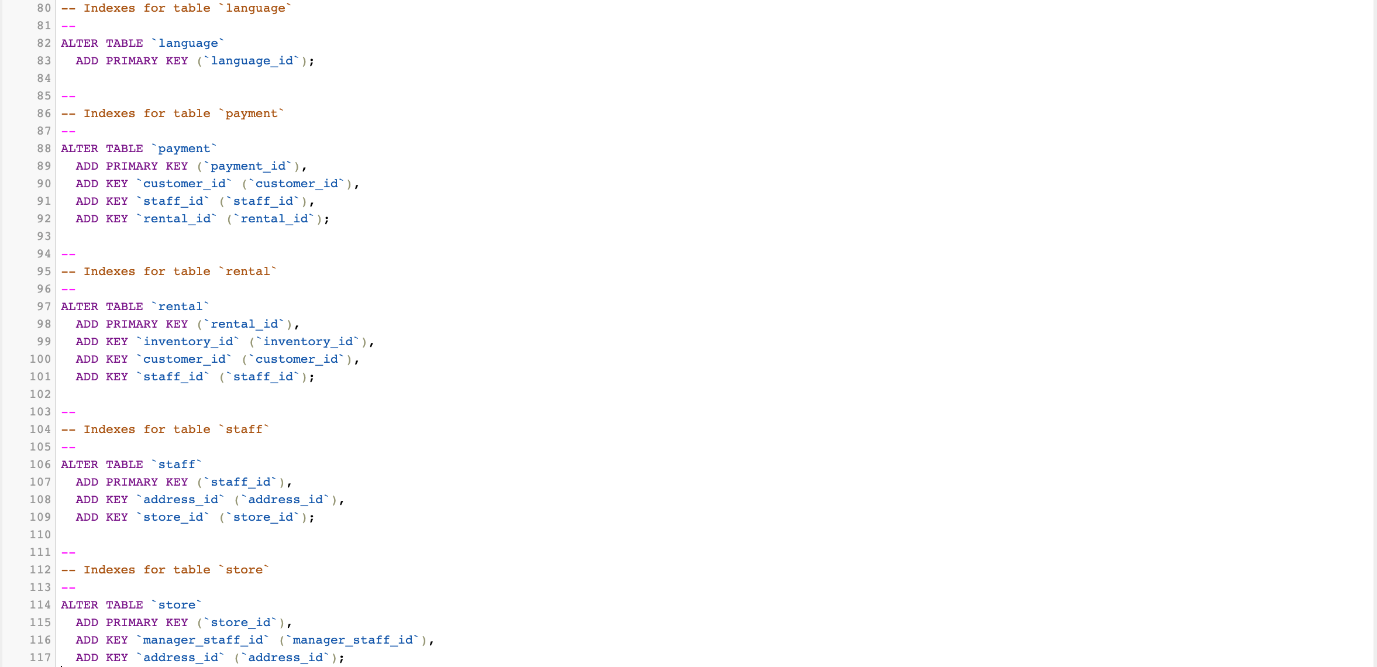
\includegraphics[width=\textwidth]{tableindexkeys3}
	\end{figure}	

\section{Table Structures}
	\begin{figure}[H]
		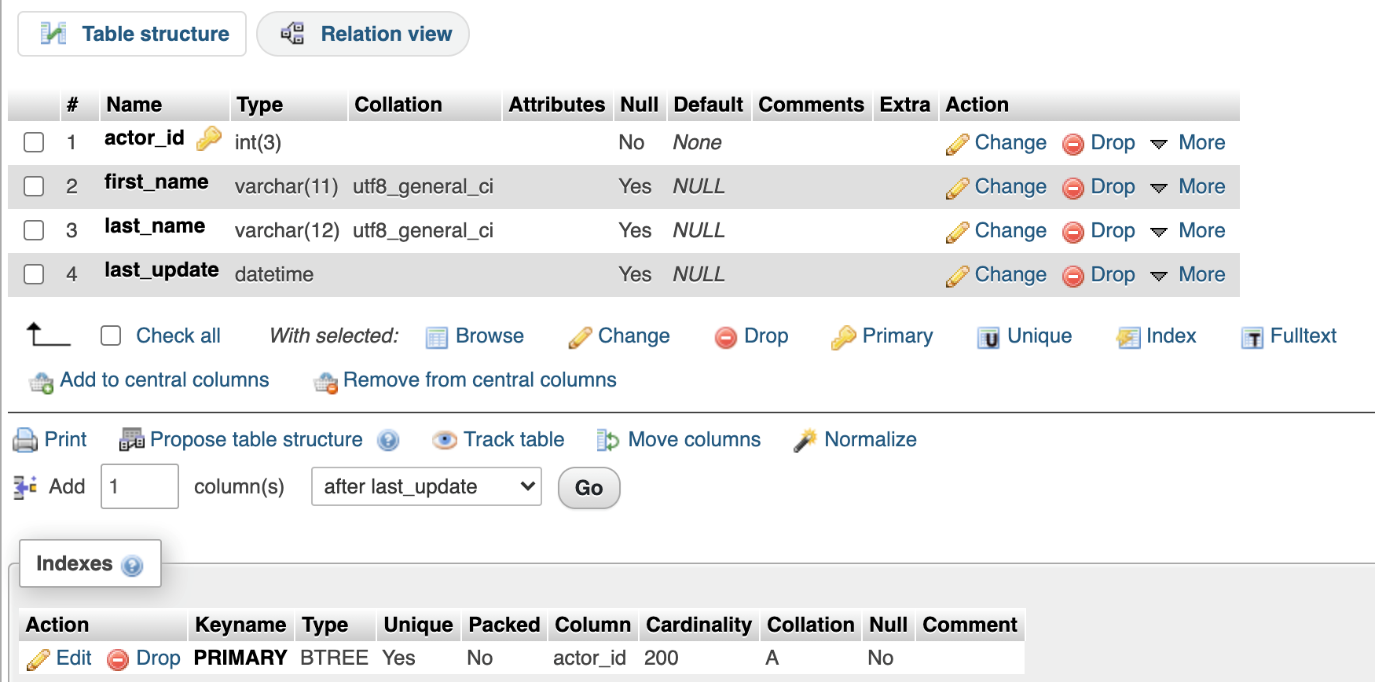
\includegraphics[width=\textwidth]{table_actor_struct}
		\caption{Structure of table "Actor"}	
	\end{figure}
	\begin{figure}[H]
		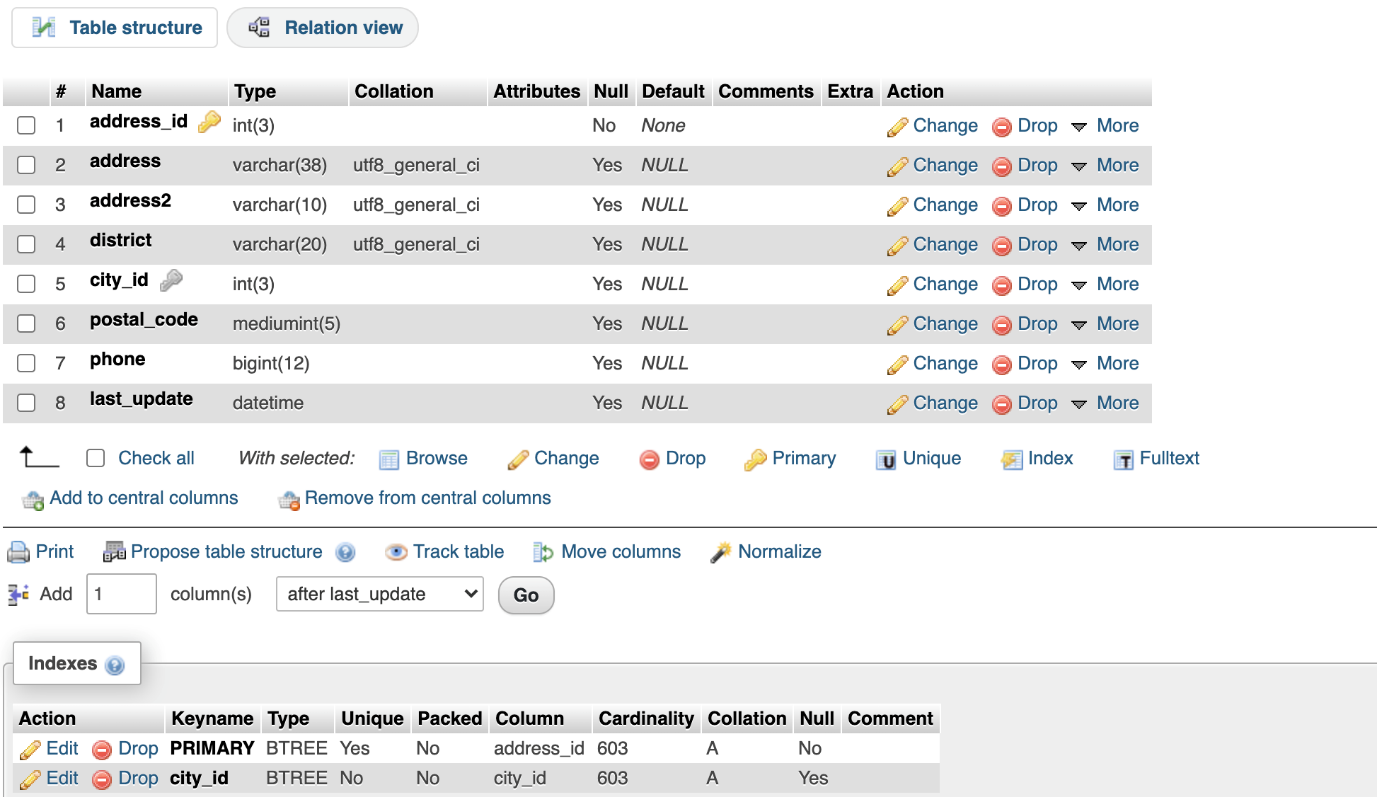
\includegraphics[width=\textwidth]{table_address_struct}
		\caption{Structure of table "Address"}	
	\end{figure}
	\begin{figure}[H]
		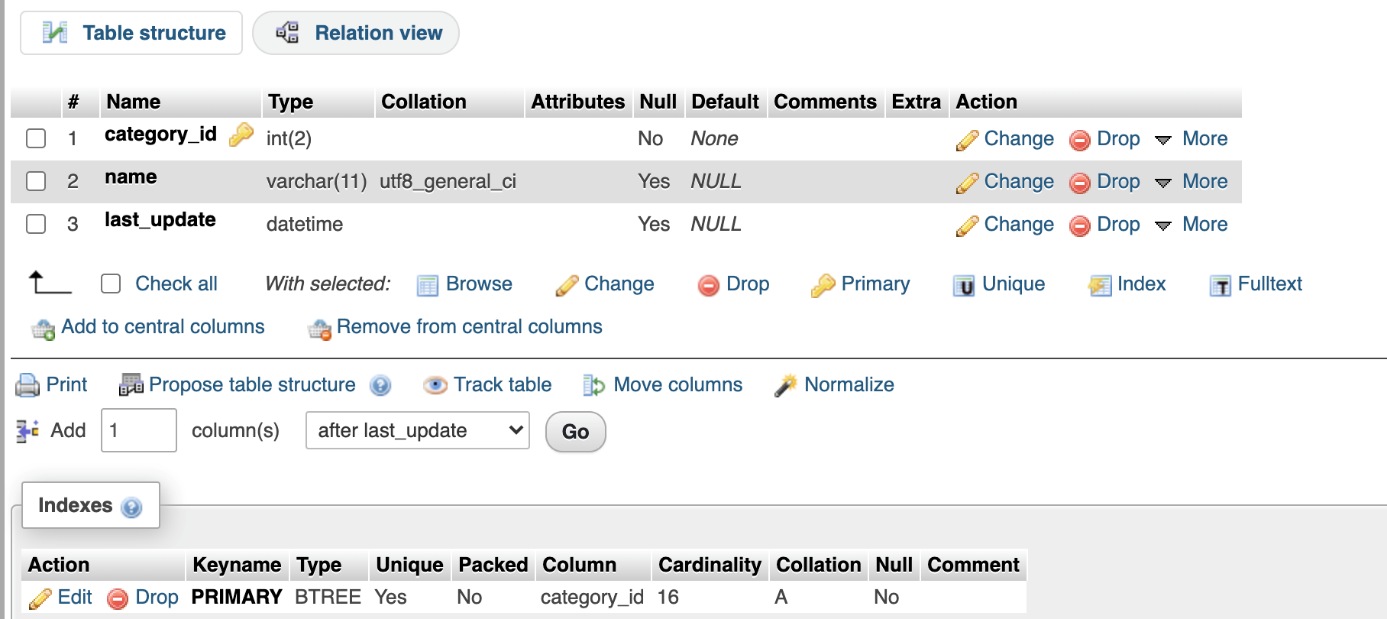
\includegraphics[width=\textwidth]{table_category_struct}
		\caption{Structure of table "Category"}	
	\end{figure}
	\begin{figure}[H]
		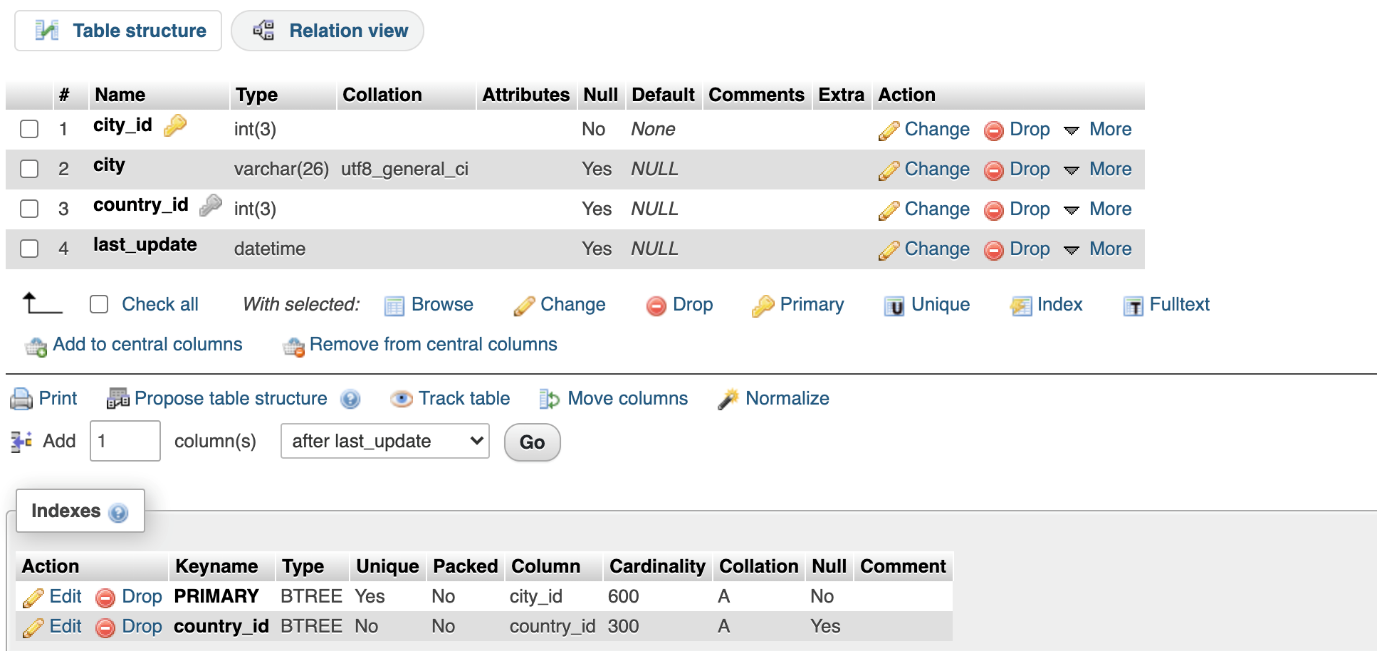
\includegraphics[width=\textwidth]{table_city_struct}
		\caption{Structure of table "City"}	
	\end{figure}
	\begin{figure}[H]
		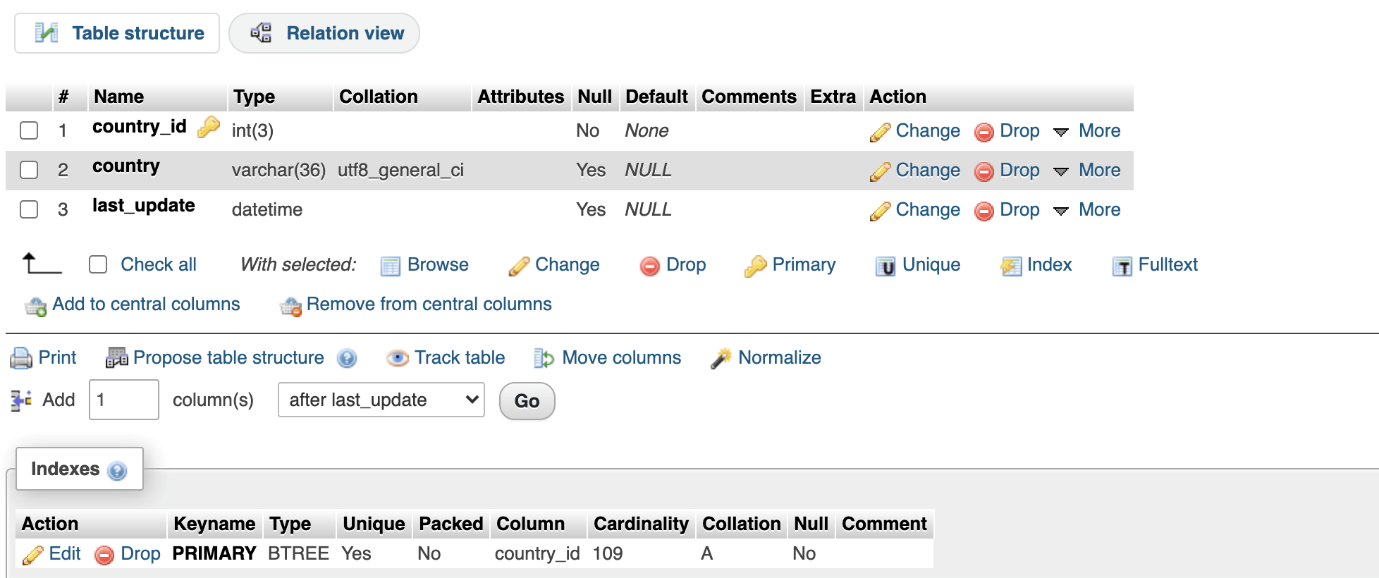
\includegraphics[width=\textwidth]{table_country_struct}
		\caption{Structure of table "Country"}	
	\end{figure}
	\begin{figure}[H]
		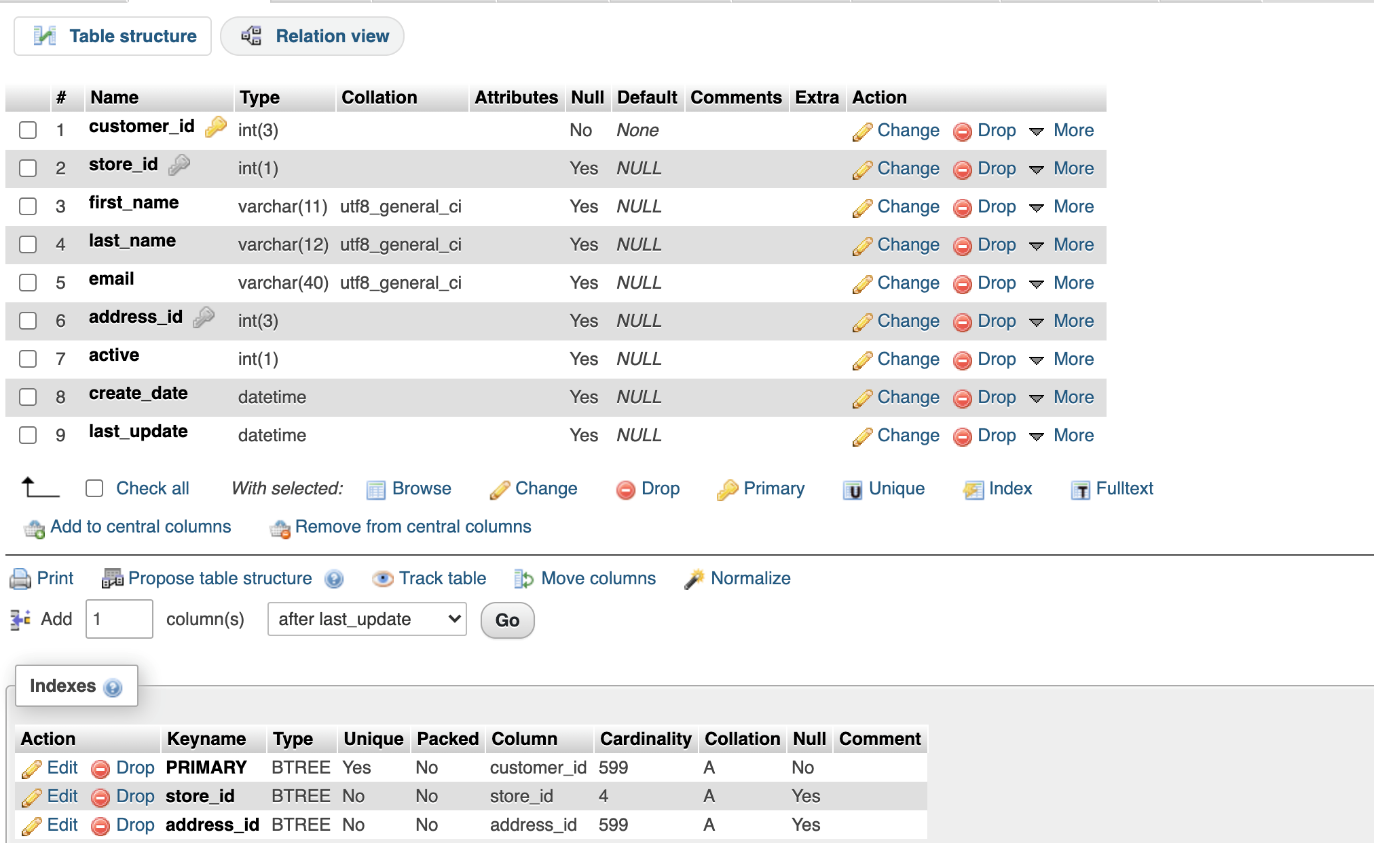
\includegraphics[width=\textwidth]{table_customer_struct}
		\caption{Structure of table "Customer"}	
	\end{figure}
	\begin{figure}[H]
		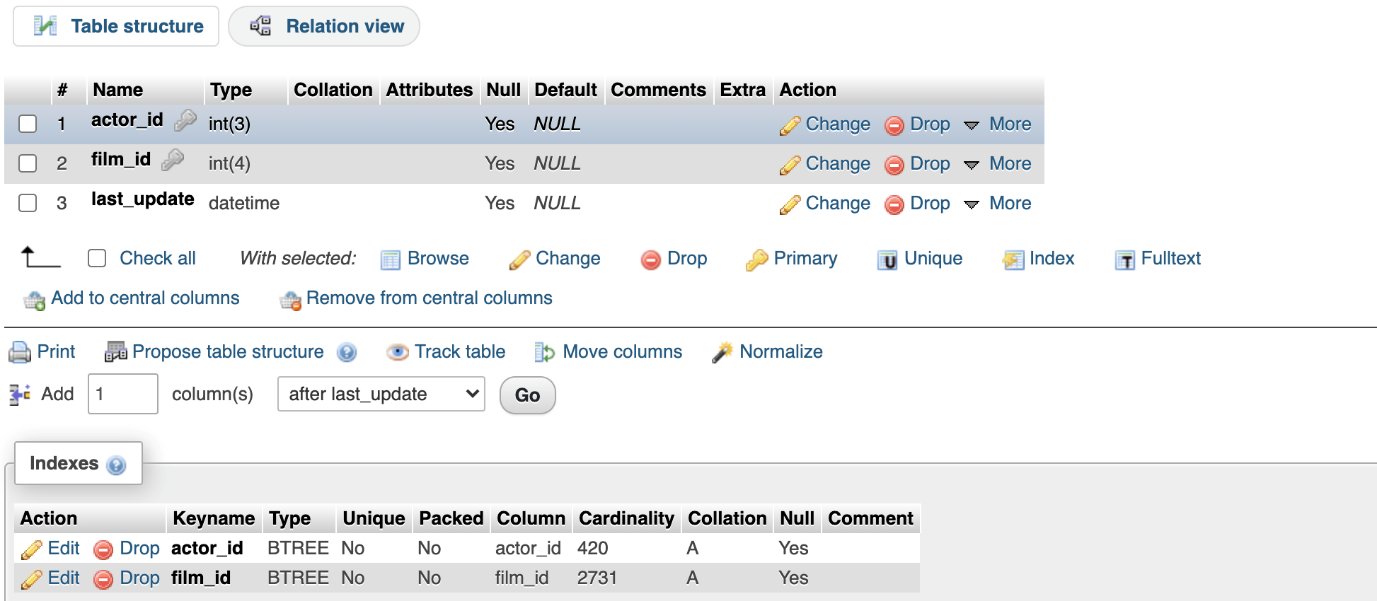
\includegraphics[width=\textwidth]{table_filmactor_struct}
		\caption{Structure of table "Film\textunderscore Actor"}	
	\end{figure}
	\begin{figure}[H]
		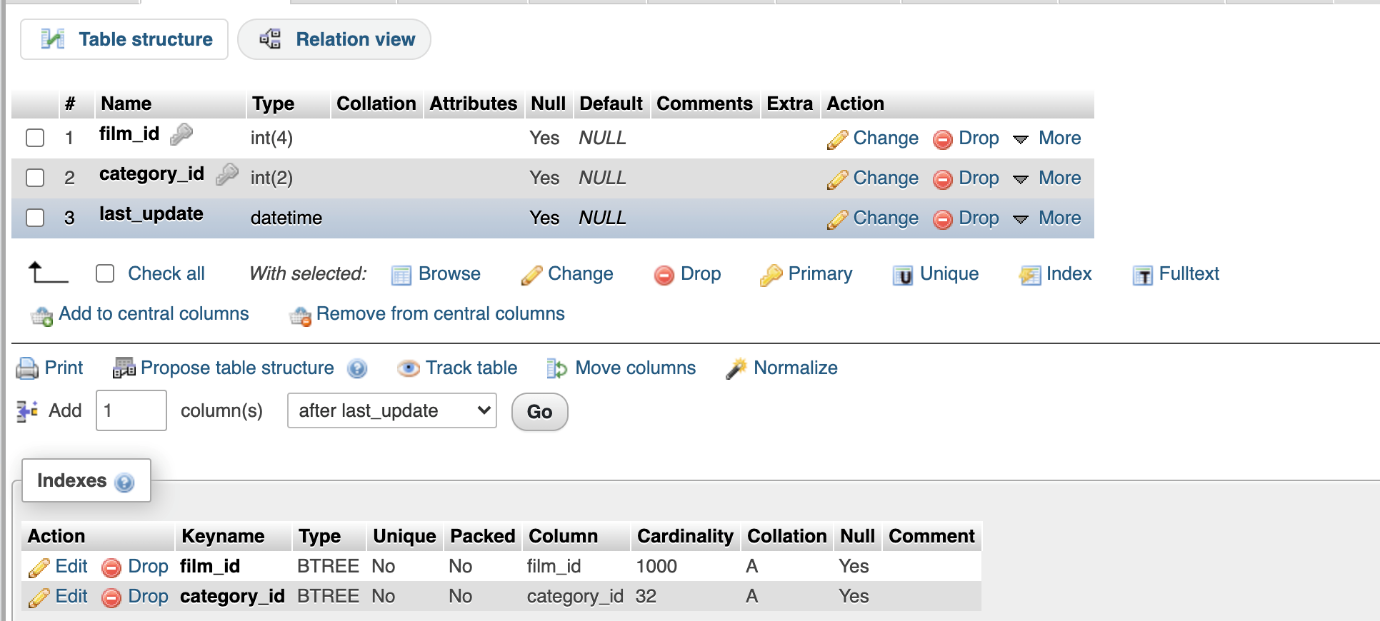
\includegraphics[width=\textwidth]{table_filmcategory_struct}
		\caption{Structure of table "Film\textunderscore Category"}	
	\end{figure}
	\begin{figure}[H]
		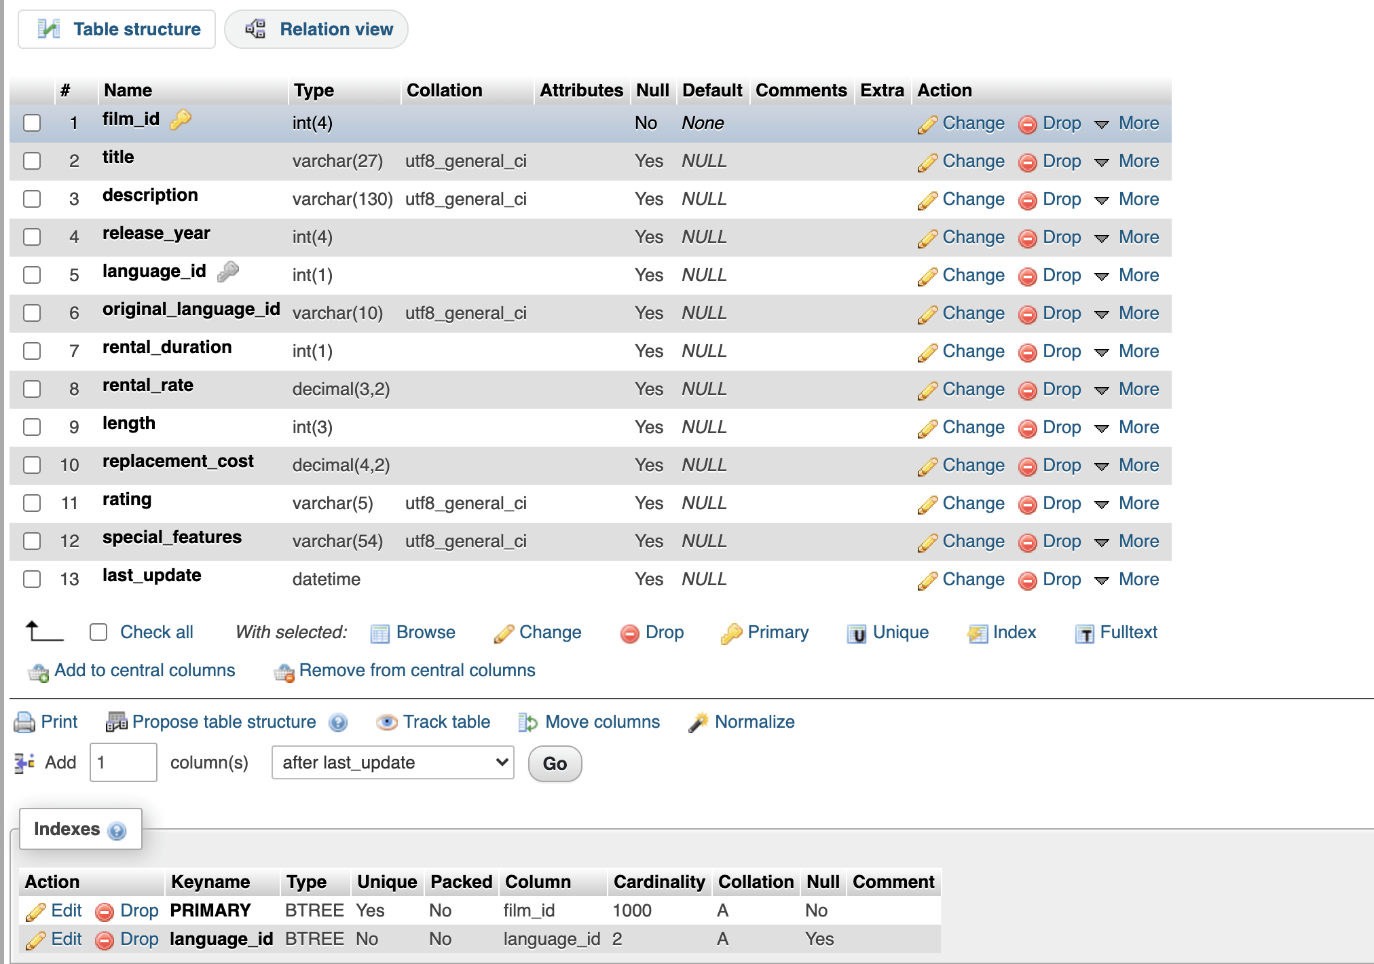
\includegraphics[width=\textwidth]{table_film_struct}
		\caption{Structure of table "Film"}	
	\end{figure}
	\begin{figure}[H]
		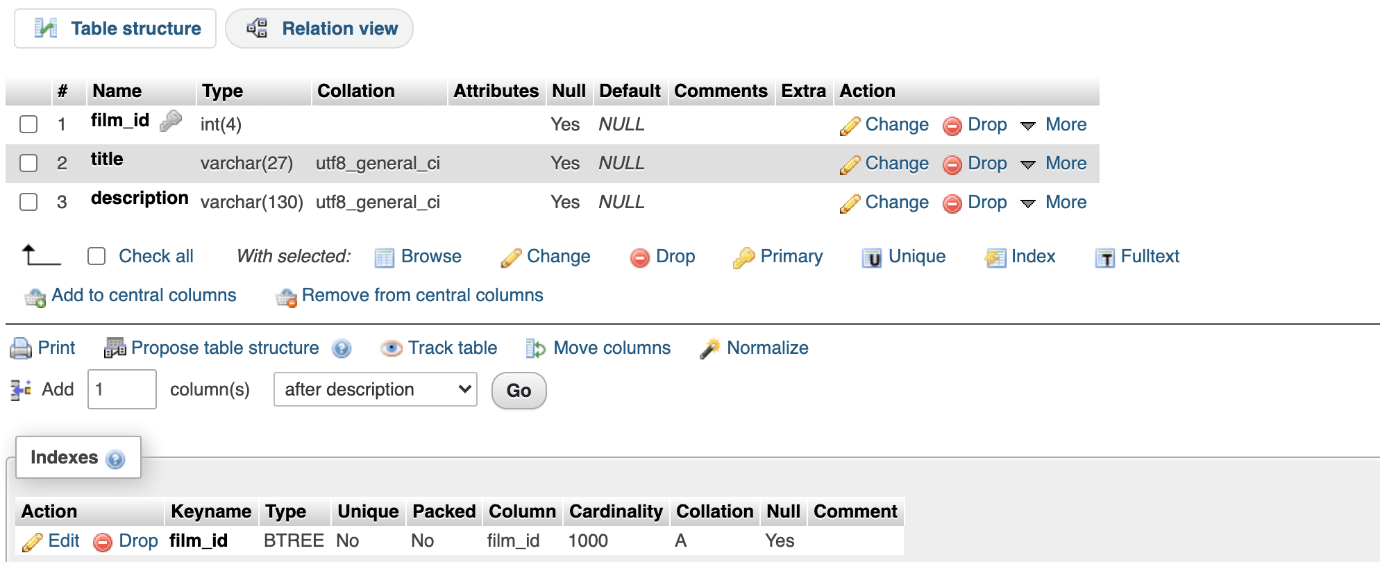
\includegraphics[width=\textwidth]{table_filmtext_struct}
		\caption{Structure of table "Film\textunderscore Text"}	
	\end{figure}
	\begin{figure}[H]
		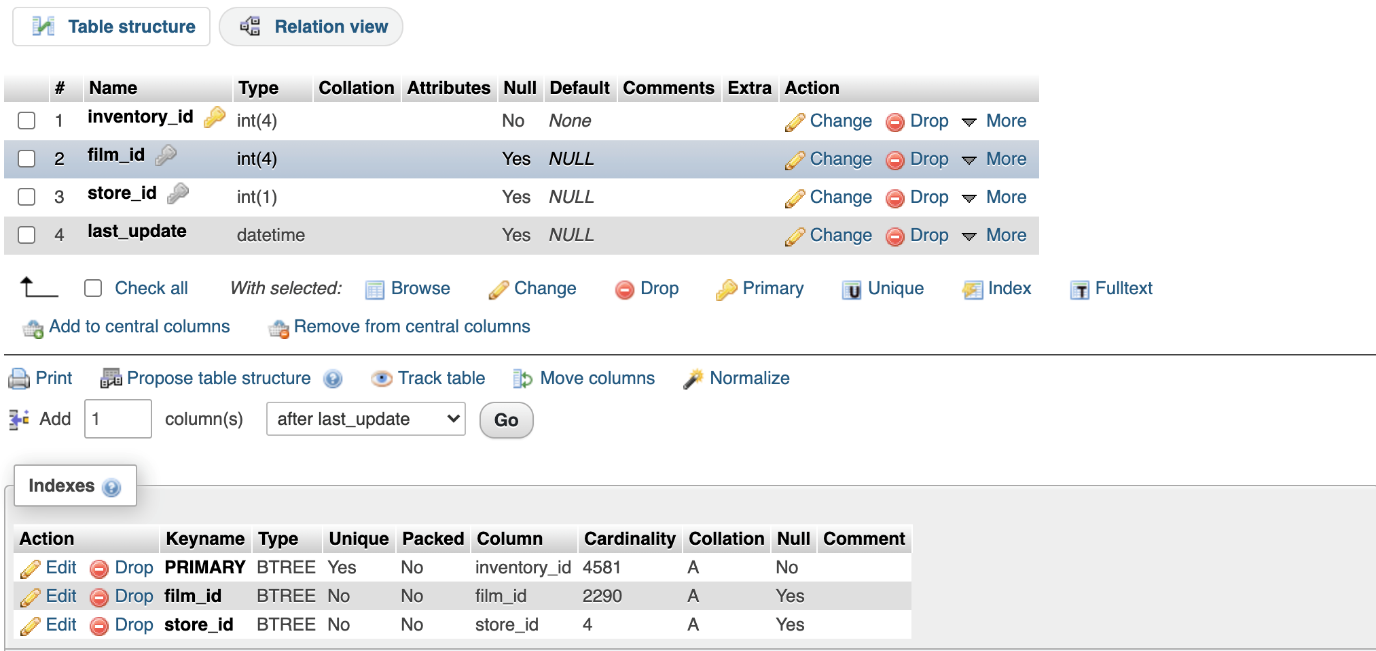
\includegraphics[width=\textwidth]{table_inventory_struct}
		\caption{Structure of table "Inventory"}	
	\end{figure}
	\begin{figure}[H]
		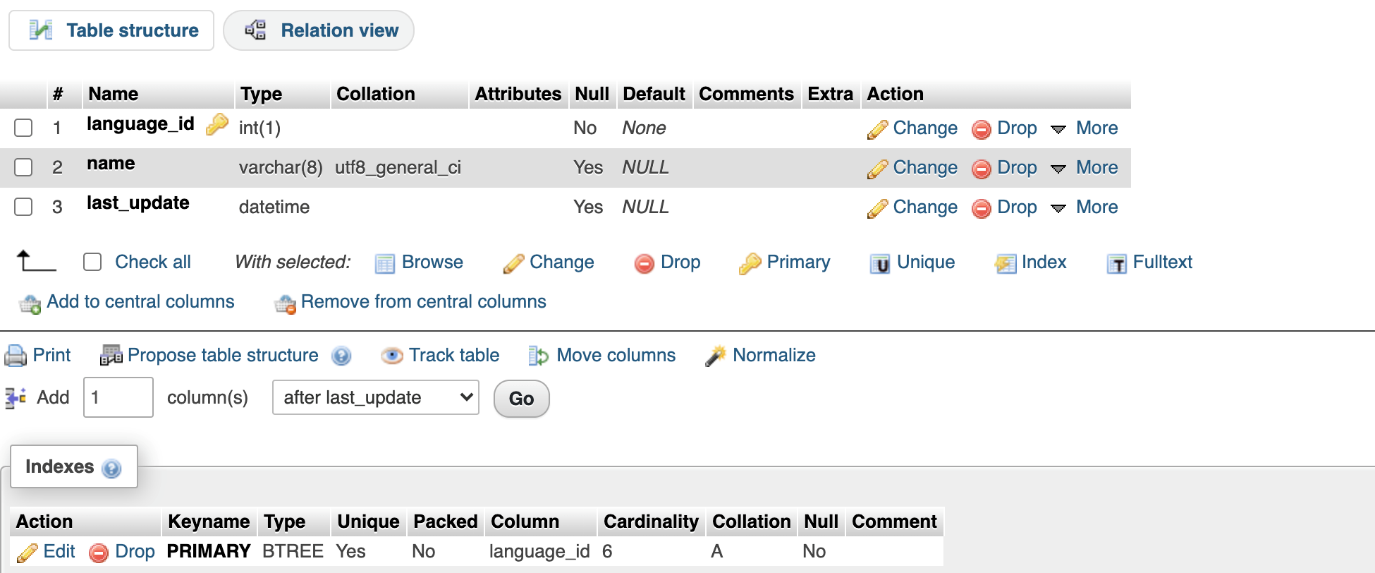
\includegraphics[width=\textwidth]{table_language_struct}
		\caption{Structure of table "Language"}	
	\end{figure}
	\begin{figure}[H]
		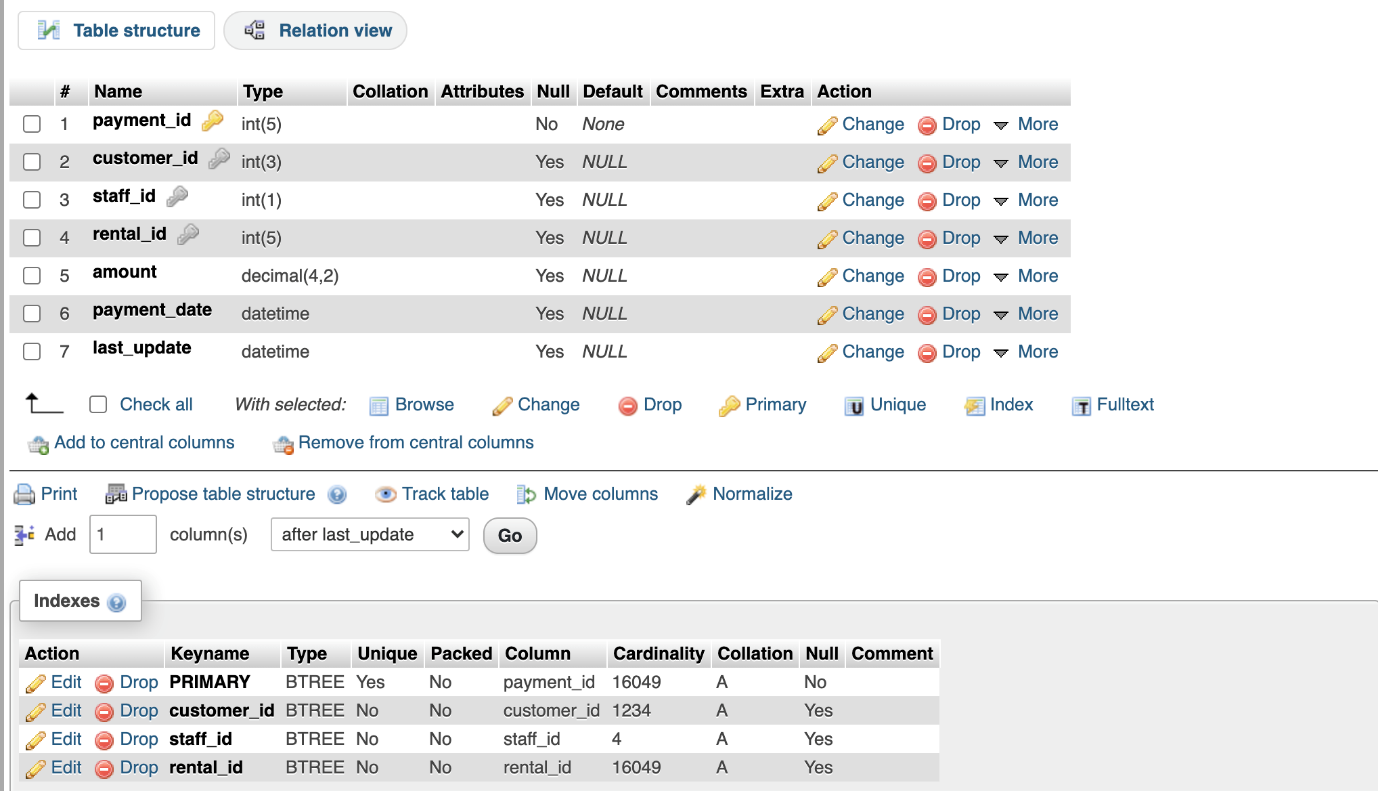
\includegraphics[width=\textwidth]{table_payment_struct}
		\caption{Structure of table "Payment"}	
	\end{figure}
	\begin{figure}[H]
		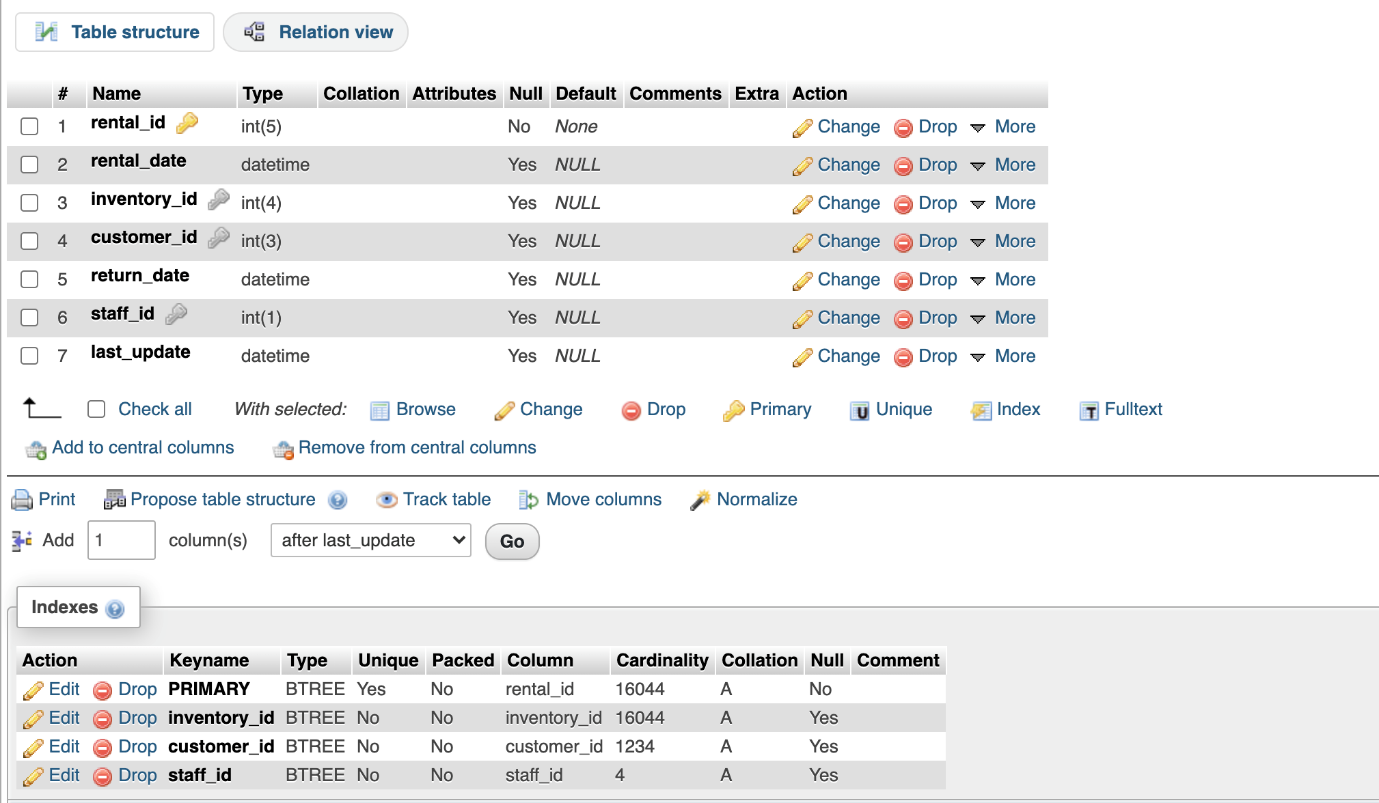
\includegraphics[width=\textwidth]{table_rental_struct}
		\caption{Structure of table "Rental"}	
	\end{figure}
	\begin{figure}[H]
		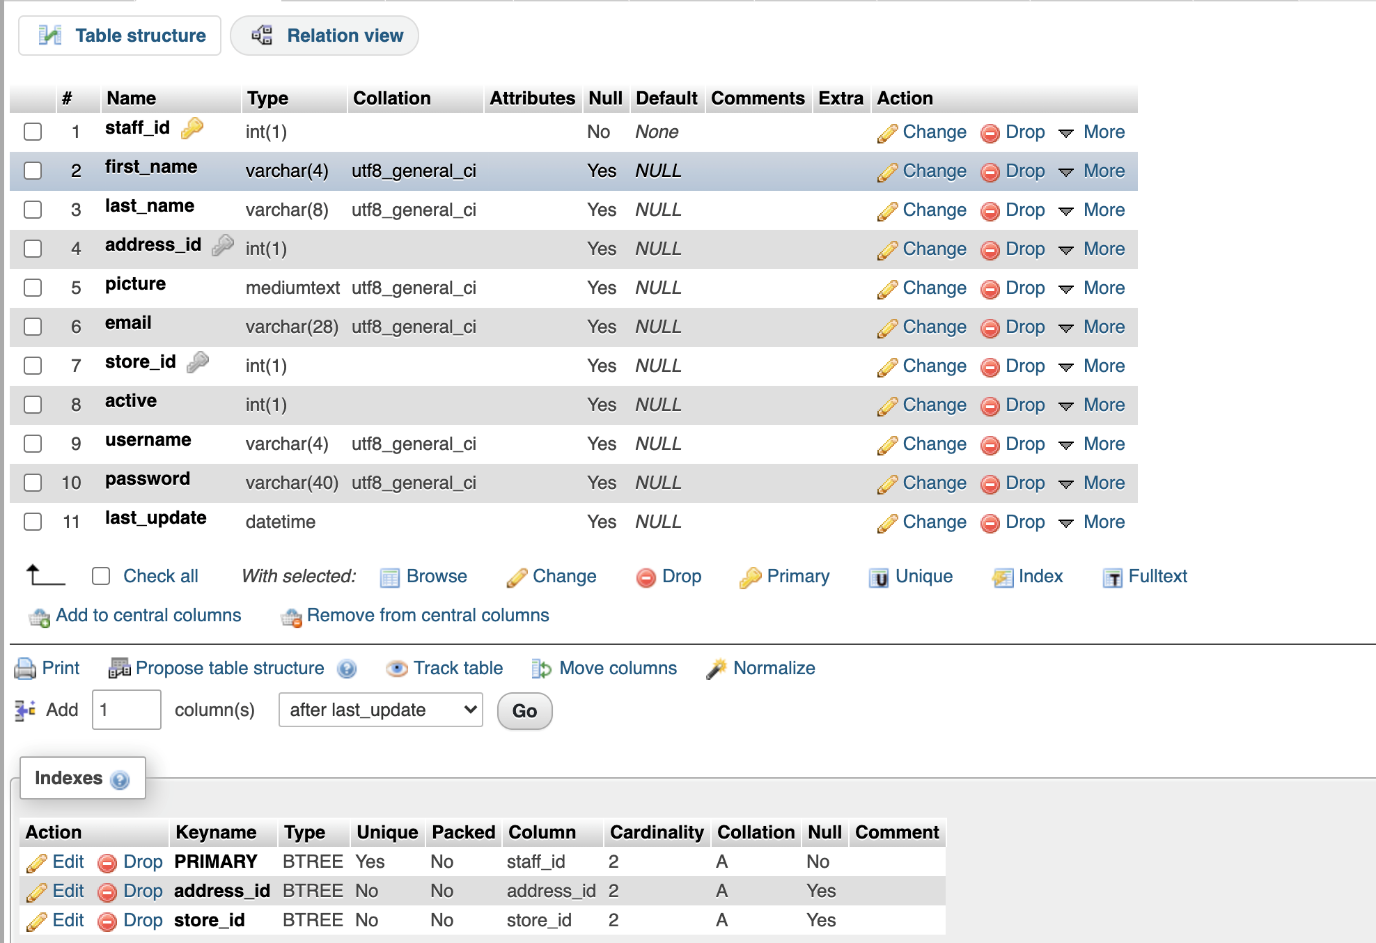
\includegraphics[width=\textwidth]{table_staff_struct}
		\caption{Structure of table "Staff"}	
	\end{figure}
	\begin{figure}[H]
		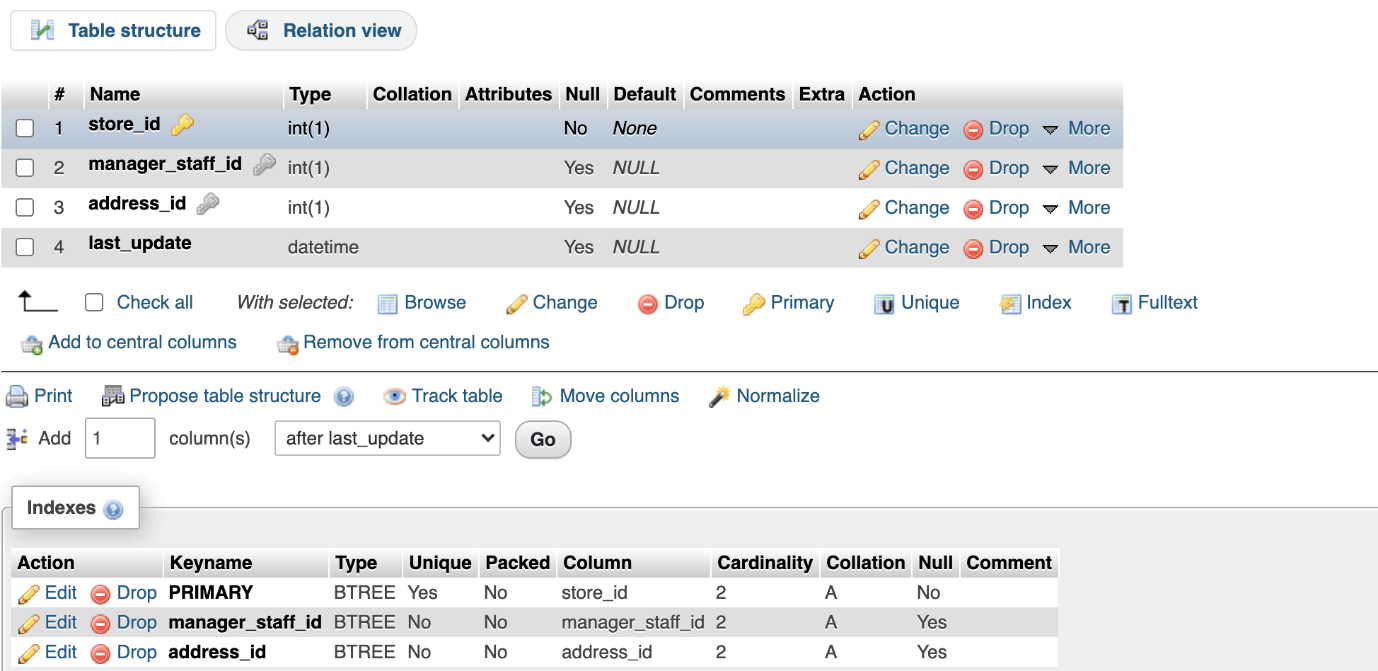
\includegraphics[width=\textwidth]{table_store_struct}
		\caption{Structure of table "Store"}	
	\end{figure}

\section{Final Results of Data Insertion \& Selection}
	\begin{figure}[H]
		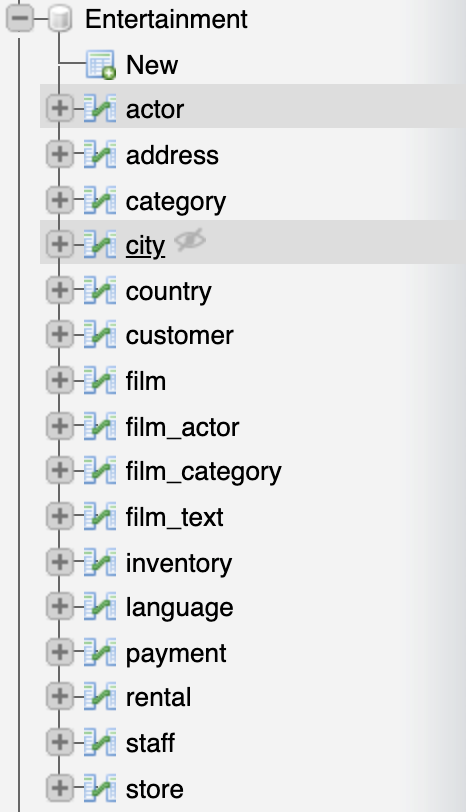
\includegraphics[width=\textwidth]{data_insertion_selection}
	\end{figure}	

\section{Overview on Tables of Database "Entertainment"}
	\begin{figure}[H]
		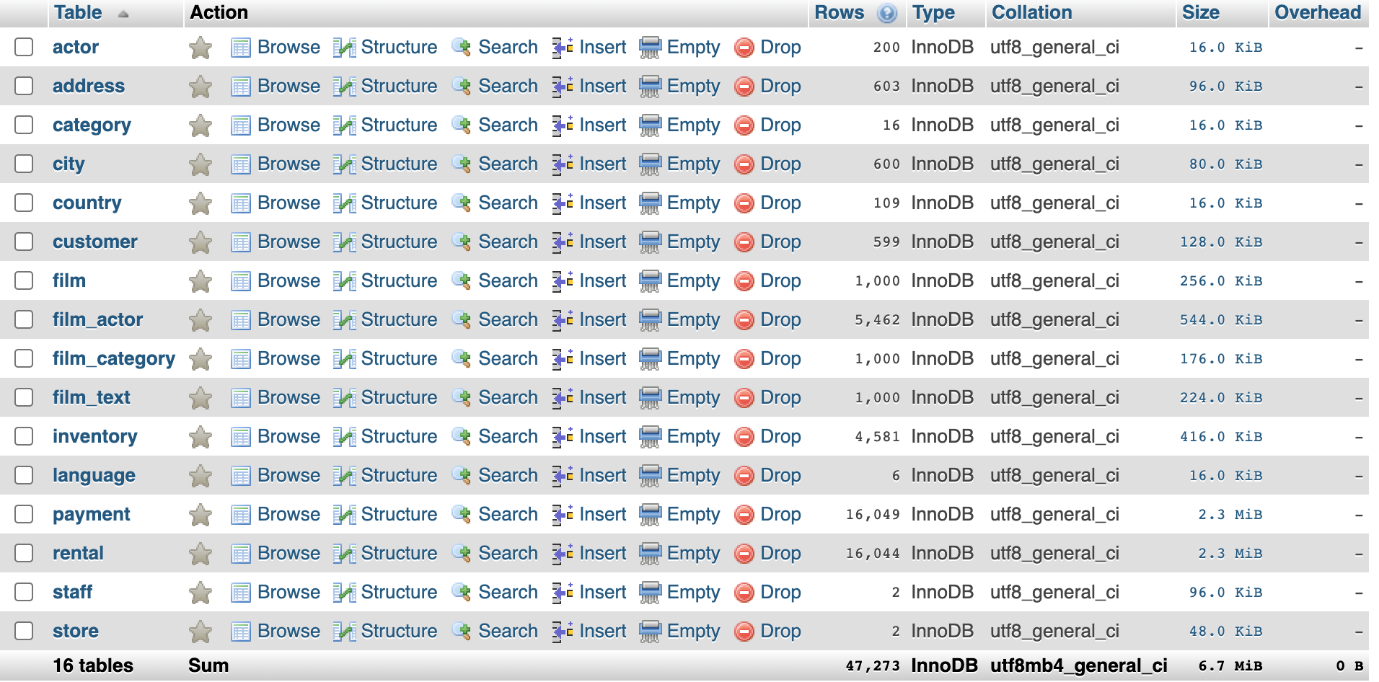
\includegraphics[width=\textwidth]{table_overview}
		\caption{Summary of tables within the database.}
	\end{figure}	
	
	\subsection{Table Contents}
		\begin{figure}[H]
			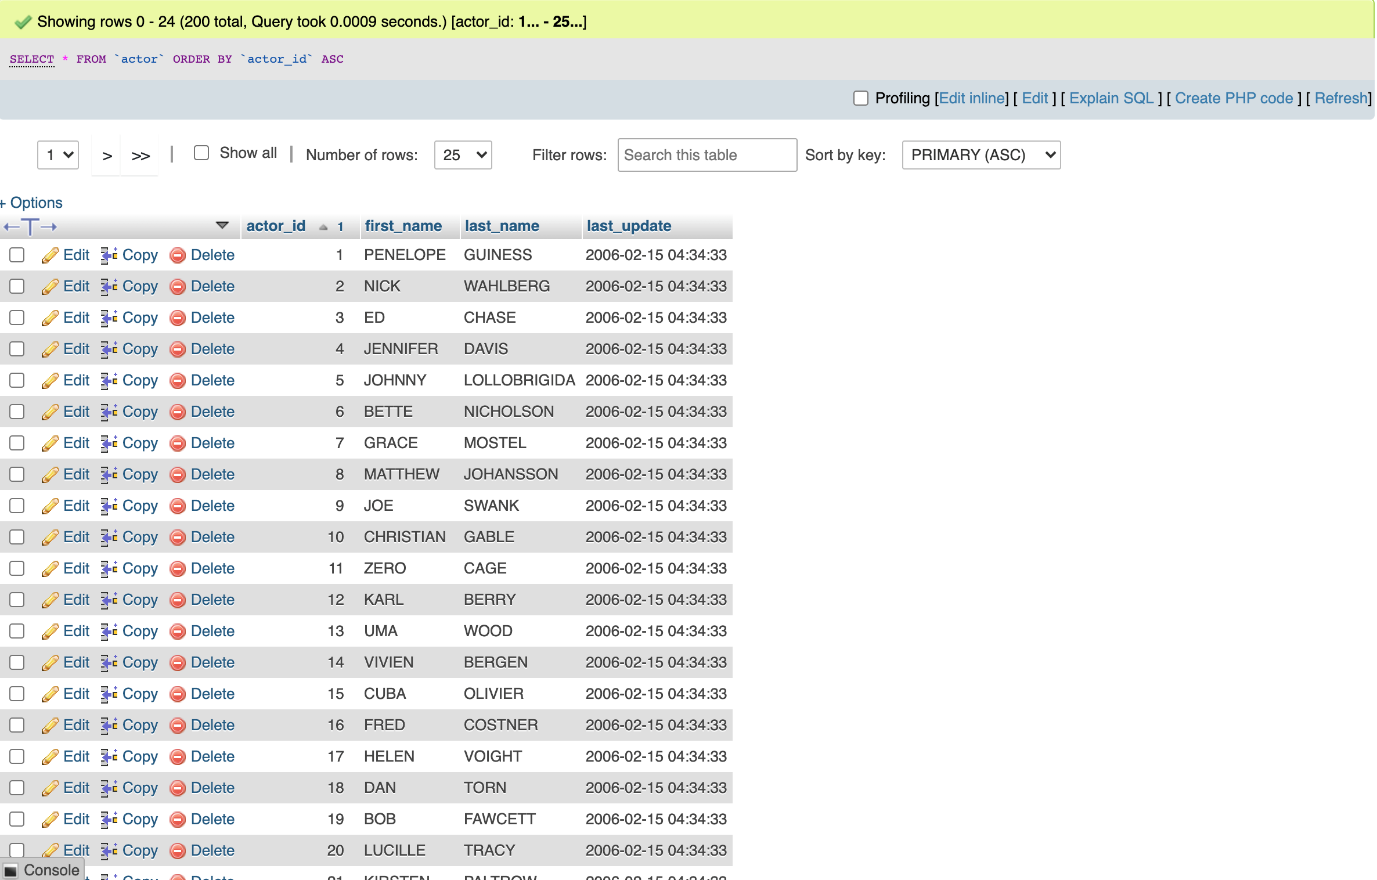
\includegraphics[width=\textwidth]{actor_content}
			\caption{Sample content of the table "Actor".}
		\end{figure}
		\begin{figure}[H]
			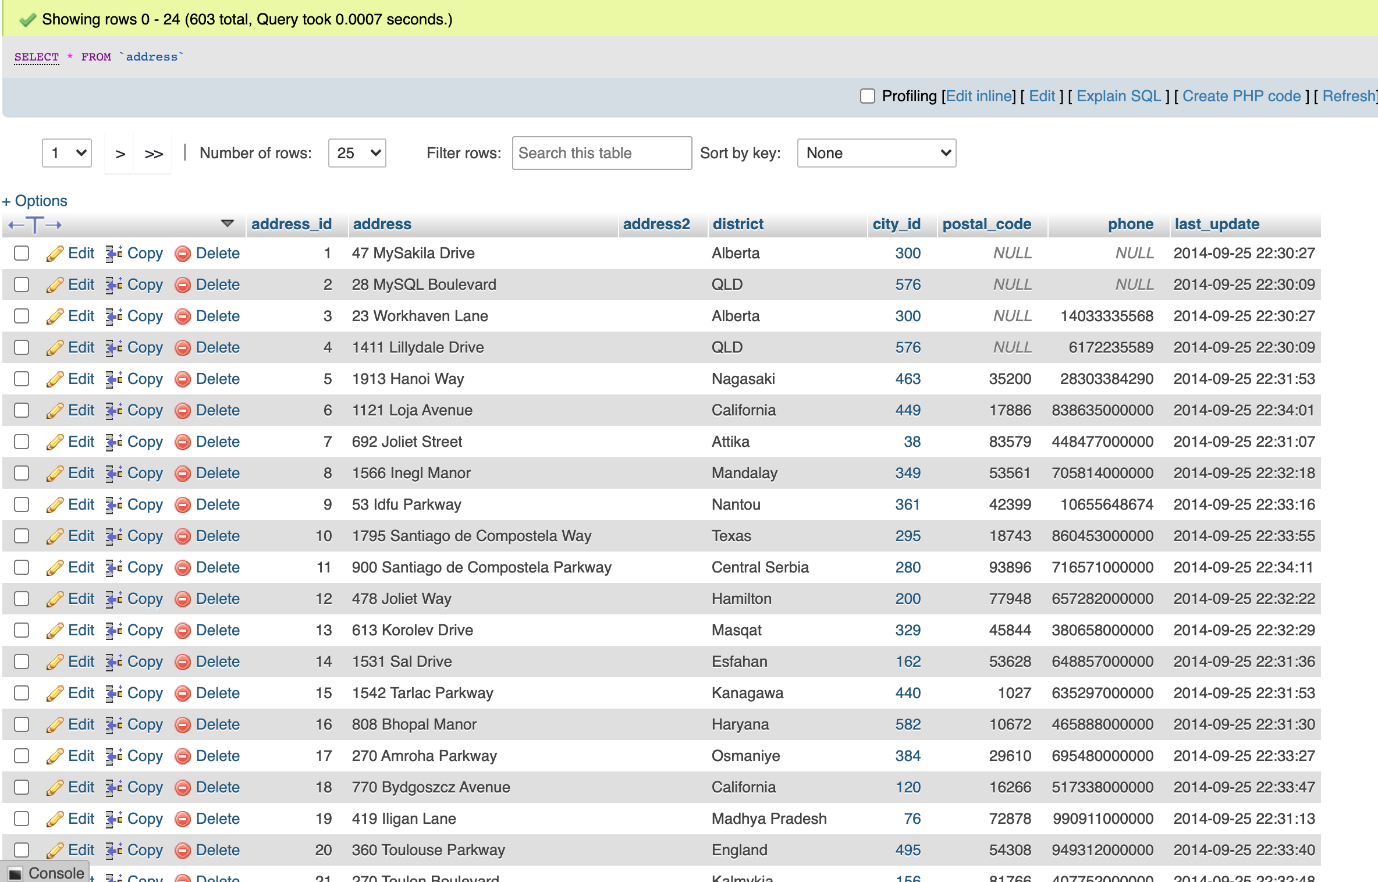
\includegraphics[width=\textwidth]{address_content}
			\caption{Sample content of the table "Address".}
		\end{figure}
		\begin{figure}[H]
			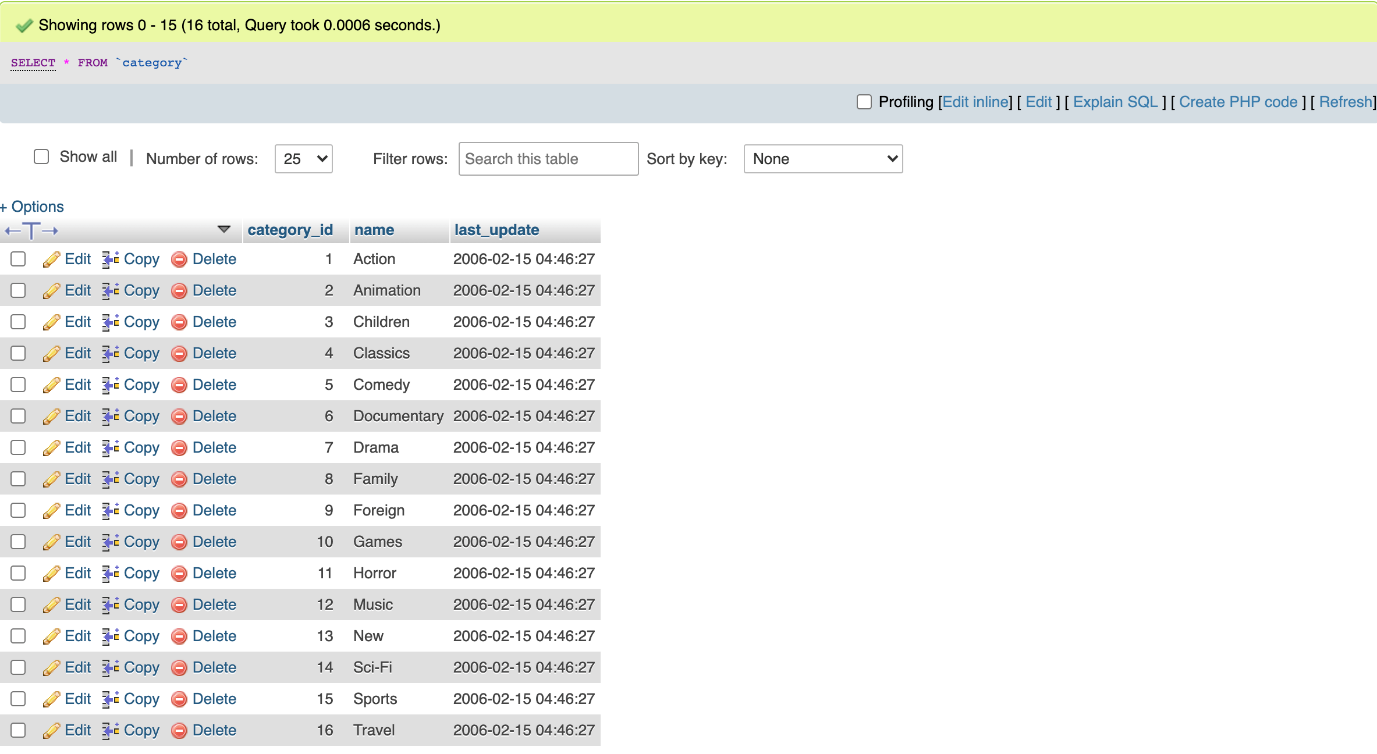
\includegraphics[width=\textwidth]{category_content}
			\caption{Sample content of the table "Category".}
		\end{figure}
		\begin{figure}[H]
			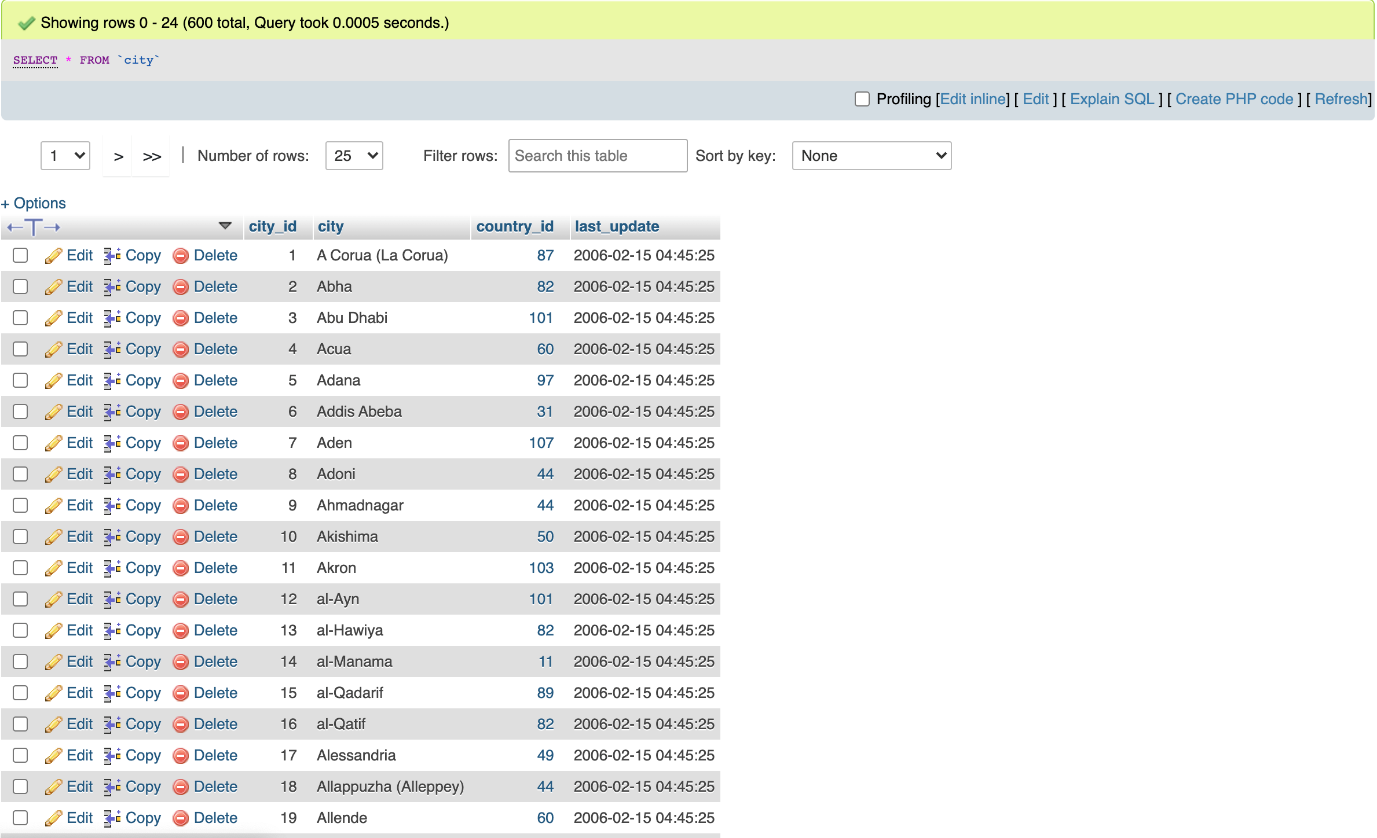
\includegraphics[width=\textwidth]{city_content}
			\caption{Sample content of the table "City".}
		\end{figure}
		\begin{figure}[H]
			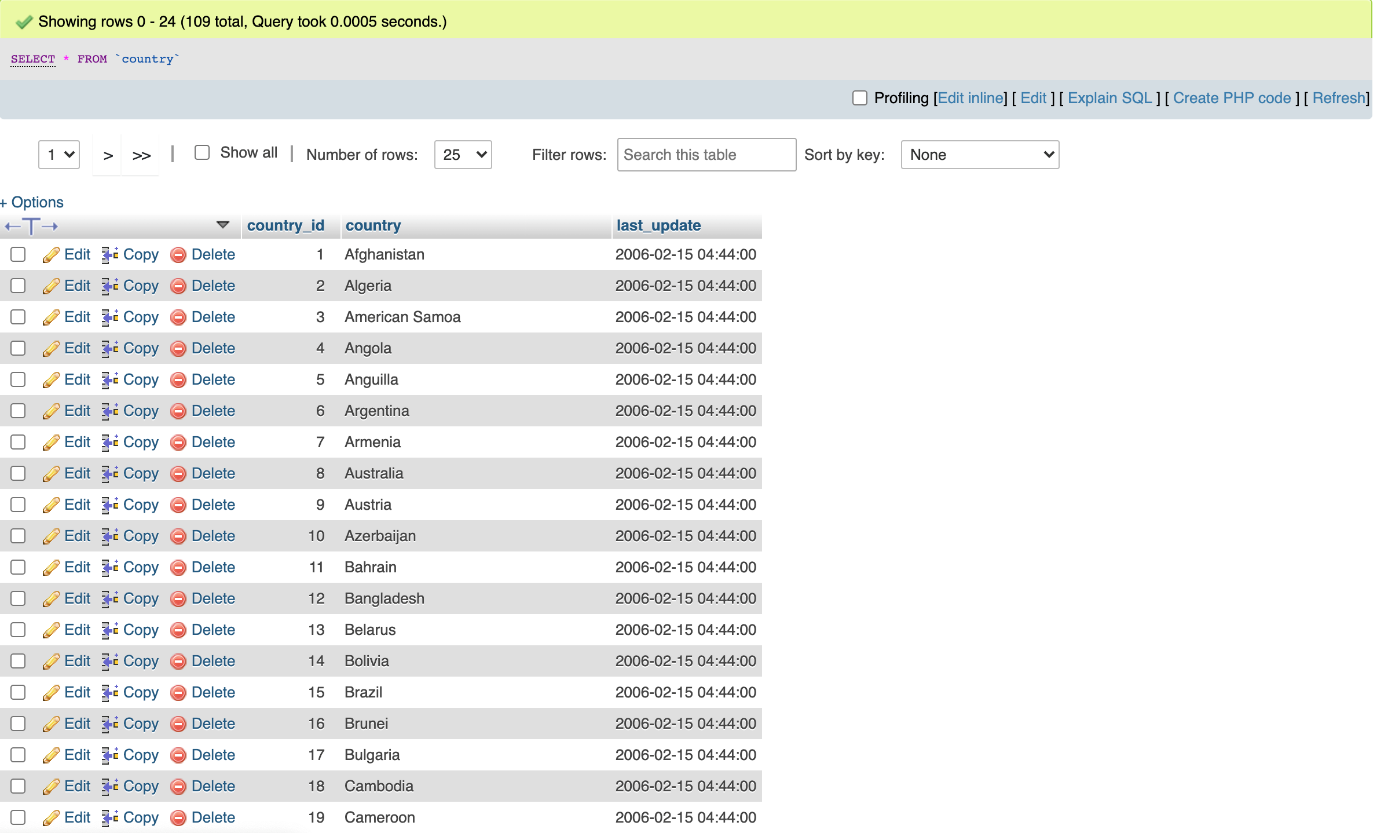
\includegraphics[width=\textwidth]{country_content}
			\caption{Sample content of the table "Country".}
		\end{figure}
		\begin{figure}[H]
			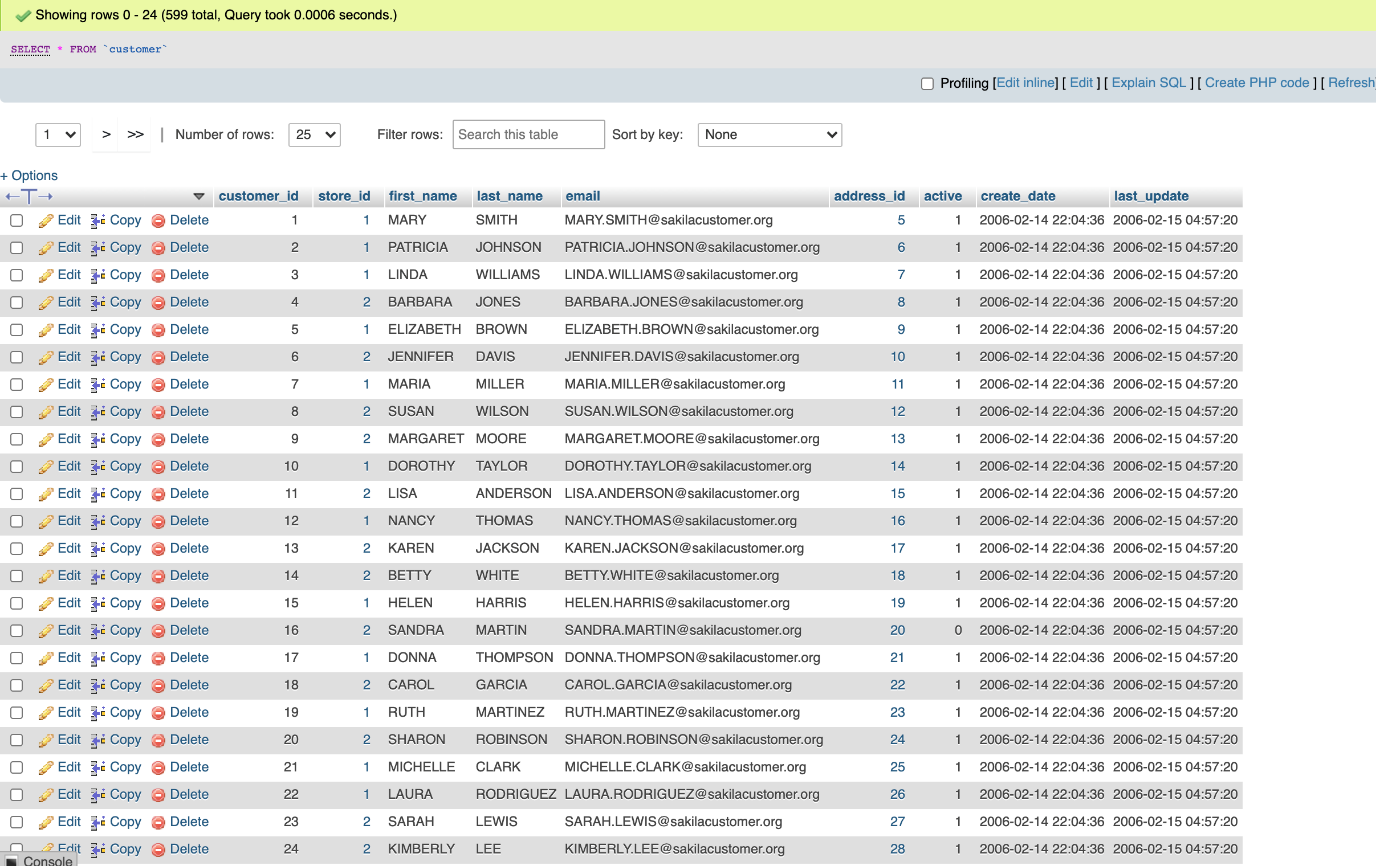
\includegraphics[width=\textwidth]{customer_content}
			\caption{Sample content of the table "Customer".}
		\end{figure}
		\begin{figure}[H]
			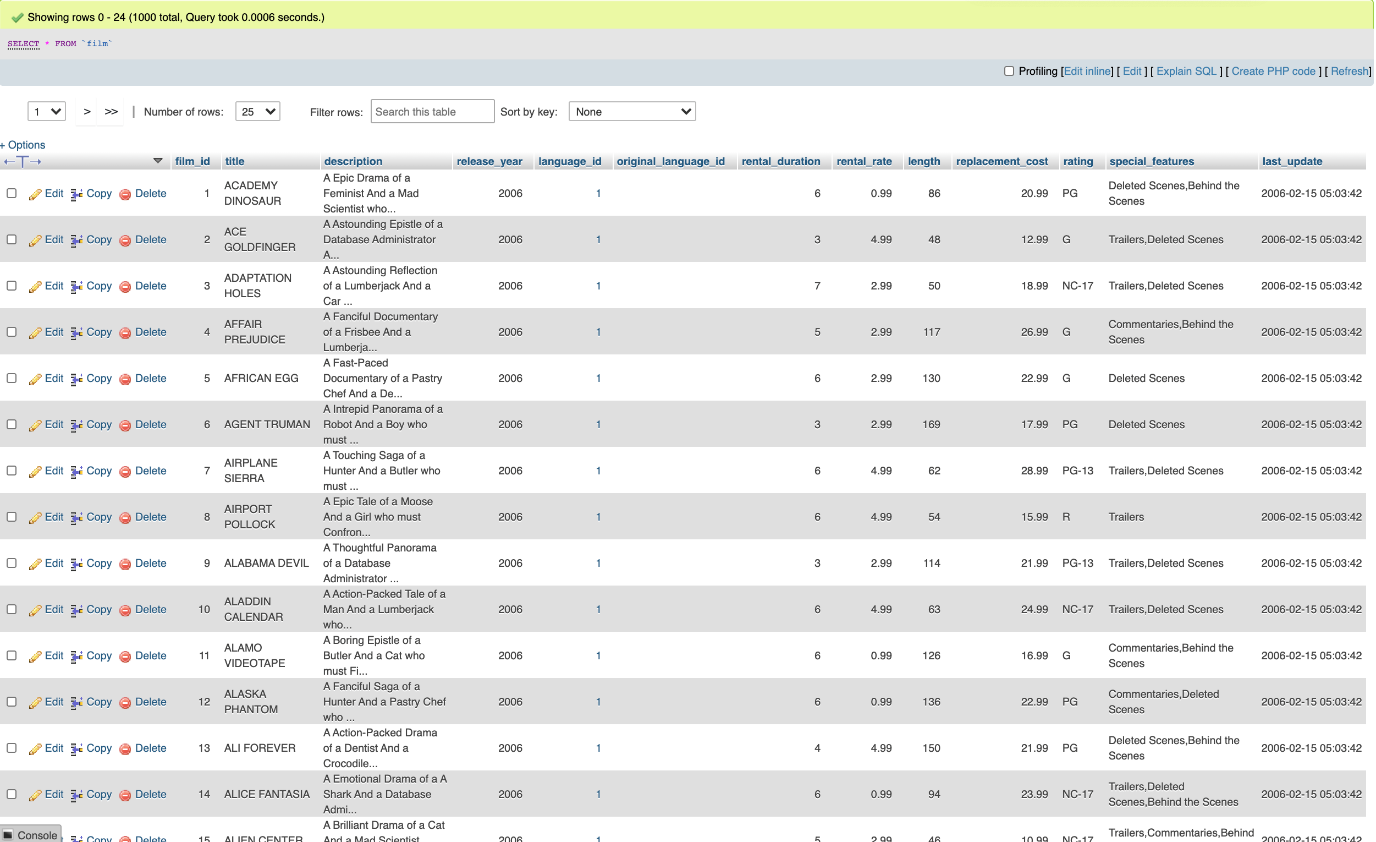
\includegraphics[width=\textwidth]{film_content}
			\caption{Sample content of the table "Film".}
		\end{figure}
		\begin{figure}[H]
			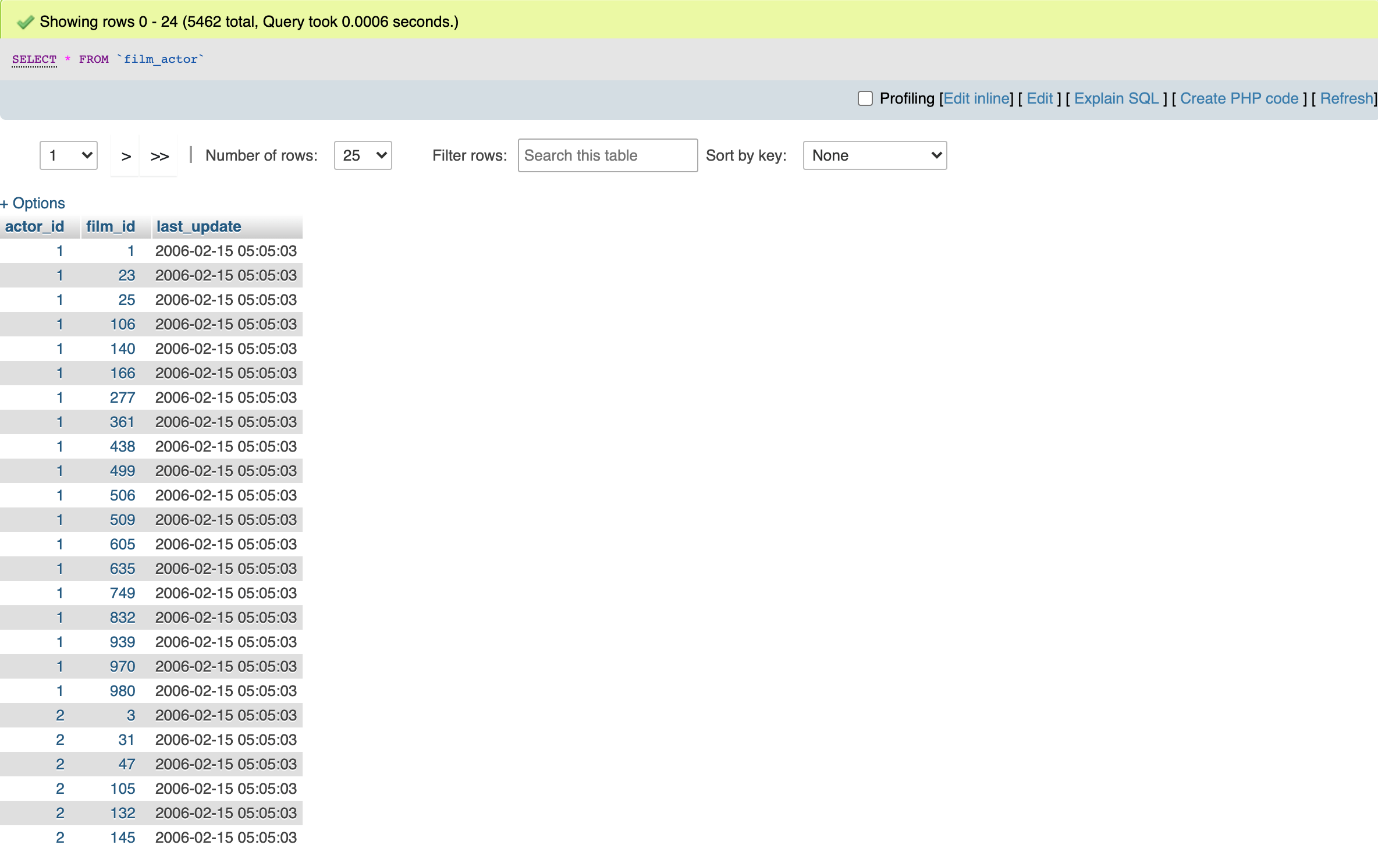
\includegraphics[width=\textwidth]{filmactor_content}
			\caption{Sample content of the table "Film\textunderscore Actor".}
		\end{figure}
		\begin{figure}[H]
			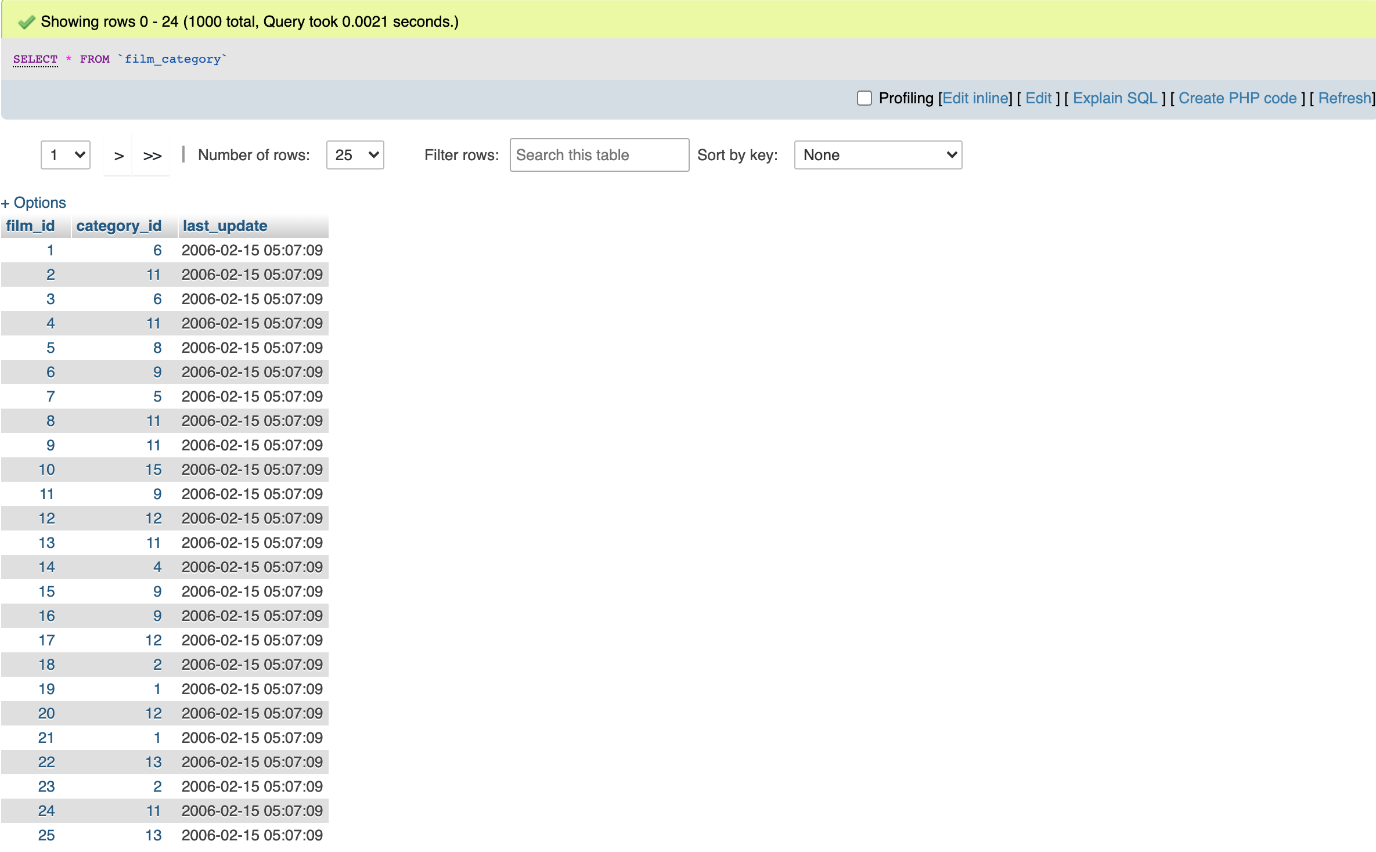
\includegraphics[width=\textwidth]{filmcategory_content}
			\caption{Sample content of the table "Film\textunderscore Category".}
		\end{figure}
		\begin{figure}[H]
			\includegraphics[width=\textwidth]{filmtext_content}
			\caption{Sample content of the table "Film\textunderscore Text".}
		\end{figure}
		\begin{figure}[H]
			\includegraphics[width=\textwidth]{inventory_content}
			\caption{Sample content of the table "Inventory".}
		\end{figure}
		\begin{figure}[H]
			\includegraphics[width=\textwidth]{language_content}
			\caption{Sample content of the table "Language".}
		\end{figure}
		\begin{figure}[H]
			\includegraphics[width=\textwidth]{payment_content}
			\caption{Sample content of the table "Payment".}
		\end{figure}
		\begin{figure}[H]
			\includegraphics[width=\textwidth]{rental_content}
			\caption{Sample content of the table "Rental".}
		\end{figure}
		\begin{figure}[H]
			\includegraphics[width=\textwidth]{staff_content}
			\caption{Sample content of the table "Staff".}
		\end{figure}
		\begin{figure}[H]
			\includegraphics[width=\textwidth]{store_content}
			\caption{Sample content of the table "Store".}
		\end{figure}

\section{Normalization}
	\subsection{Entity Relation Diagram After Normalization}
		\begin{figure}[H]
			\includegraphics[width=\textwidth]{er_normalized}
			\caption{Database structure after normalization.}
		\end{figure}

	\subsection{Tables Affected by Normalization}
		The tables Film\textunderscore Special\textunderscore Features is normalized from the Film table to preserve compliance with the First Normal Form. 
		\begin{figure}[H]
			\includegraphics[height = \textheight]{table_filmspecialfeatures_norm}
			\caption{Table "Film\textunderscore Special\textunderscore Features", normalized.}
		\end{figure}

		The District, City and Address tables have been recompiled after normalization. \\\\
		The field last\textunderscore update is retained for the purpose of easing maintenance of the altered tables. \\\\
		It can be noted that for the Address and City tables, many errors within the database have been uncovered due to the use of normalization that otherwise would have gone unnoticed.  Errors found include: 
		\begin{itemize}
			\item Cities with ID 121, 493 and 583 not having a listed district. Their district\textunderscore id fields in the newly reorganized City table have been left blank.
			\item Entry with city\textunderscore id 313 in the City table not existing within the address table. district\textunderscore id field of this city also left blank in the City table.
			\item Multiple occurences of the same city\textunderscore id being in multiple districts in the address table. To preserve database integrity after normalization, one of the extra districts is removed with the use of an SQL command containing the GROUP BY keyword. 
		\end{itemize}
		\begin{figure}[H]
			\includegraphics[width=\textwidth]{table_district_norm}
			\caption{Table "District", normalized.}
		\end{figure}
		\begin{figure}[H]
			\includegraphics[width=\textwidth]{table_address_norm}
			\caption{Table "Address", normalized.}
		\end{figure}
		\begin{figure}[H]
			\includegraphics[width=\textwidth]{table_city_norm}
			\caption{Table "City", normalized.}
		\end{figure} 
		Note that \textbf{original\textunderscore film\textunderscore id} now has a foreign key relation with the Language table to increase consistency. Its database has consequently been coverted to \textbf{int}.
		\begin{figure}[H]
			\includegraphics[width=\textwidth]{table_film_norm}
			\caption{Table "Film", normalized.}
		\end{figure}
		\begin{figure}[H]
			\includegraphics[height = 20cm]{table_filmrental_norm}
			\caption{Table "Film\textunderscore Rental", normalized.}
		\end{figure}
		\begin{figure}[H]
			\includegraphics[width=\textwidth]{table_staff_norm}
			\caption{Table "Staff", normalized.}
		\end{figure}
		\begin{figure}[H]
			\includegraphics[width=\textwidth]{table_stafflogin_norm}
			\caption{Table "Staff\textunderscore Login", newly created after normalization.}
		\end{figure}


	\subsection{Table Structures After Normalization}
		\begin{figure}[H]
			\includegraphics[width=\textwidth]{table_district_nstruct}
			\caption{Structure of table "District", normalized.}
		\end{figure}
		\begin{figure}[H]
			\includegraphics[width=\textwidth]{table_film_nstruct}
			\caption{Structure of table "Film", normalized.}
		\end{figure}
		\begin{figure}[H]
			\includegraphics[width=\textwidth]{table_filmtext_nstruct}
			\caption{Structure of table "Film\textunderscore Text", normalized.}
		\end{figure}
		\begin{figure}[H]
			\includegraphics[width=\textwidth]{table_staff_nstruct}
			\caption{Structure of table "Staff", normalized.}
		\end{figure}
		\begin{figure}[H]
			\includegraphics[width=\textwidth]{table_stafflogin_nstruct}
			\caption{Structure of table "Staff\textunderscore Login", normalized.}
		\end{figure}
	
	\subsection{Foreign Key Relations After Normalization}
		To preserve the integrity of relations inside of the database, foreign key constraints within the database have been modified based on these criterion:
		\begin{itemize}
			\item Two foreign keys have been modified with ON DELETE CASCADE as the deletion of table data involving these foreign keys will only affect this one table, and will not cascade down the entire database. The tables involved are "Film\textunderscore Actor" and "Film\textunderscore Category", which have their primary keys in the tables "Actor" and "Category" respectively. 
			\item The primary keys of three tables are left with the original ON DELETE RESTRICT constraint as these tables are central components of the entire database, and should have all deletions resolved on lower levels on the database before they themselves are allowed to be deleted. This affects all tables having a foreign key from the tables "Customer", "Film", and "Staff".
			\item Every other foreign key constraint is set to ON DELETE SET NULL by default. This is to facilitate easy reorganisation and maintenance on the database as this database contains numerous errata; having the ability to delete erroneous entries easily drastically improves the ease of managing and fixing the database.
			\item For the same reasons as above, all foreign key constraints with regards to updates have been set to ON UPDATE CASCADE. This is to accomodate the many value changes and error corrections that are expected to take place over the course of using this database. 
		\end{itemize}
		Displayed below are examples of affected foreign key relations.
		\begin{figure}[H]
			\includegraphics[width=\textwidth]{actor_cascade}
			\caption{The table "Film\textunderscore Actor" having its ON DELETE relation with "Actor" modified to CASCADE.}
		\end{figure}
		\begin{figure}[H]
			\includegraphics[width=\textwidth]{category_cascade}
			\caption{The table "Film\textunderscore Category" having its ON DELETE relation with "Category" modified to CASCADE.}
		\end{figure}
		\begin{figure}[H]
			\includegraphics[width=\textwidth]{customer_restrict}
			\caption{The table "Rental" having its ON DELETE relation with "Customer" modified to RESTRICT.}
		\end{figure}
		\begin{figure}[H]
			\includegraphics[width=\textwidth]{address_restrict}
			\caption{The table "Store" having its ON DELETE relation with "Address" modified to RESTRICT.}
		\end{figure}
		\begin{figure}[H]
			\includegraphics[width=\textwidth]{store_restrict}
			\caption{The table "Staff" having its ON DELETE relation with "Store" modified to RESTRICT.}
		\end{figure}
		\begin{figure}[H]
			\includegraphics[width=\textwidth]{film_restrict}
			\caption{The table "Film\textunderscore Text" having its ON DELETE relation with "Film" modified to RESTRICT.}
		\end{figure}
		\begin{figure}[H]
			\includegraphics[width=\textwidth]{staff_restrict}
			\caption{The table "Payment" having its ON DELETE relation with "Staff" modified to RESTRICT.}
		\end{figure}
		\begin{figure}[H]
			\includegraphics[width=\textwidth]{setnull_cascade}
			\caption{The default setting for foreign key relations with other tables in this database.}
		\end{figure}

	\subsection{Insertion After Normalization}
		\begin{figure}[H]
			\includegraphics[height=16cm]{specialfeatures11_insert}
			\caption{Insertion of new data into the table "Special\textunderscore Features" after normalization}
		\end{figure}
		\begin{figure}[H]
			\includegraphics[height=16cm]{district1_insert_norm}
			\includegraphics[width=\textwidth]{district2_insert_norm}
			\caption{Insertion of new data into the table "District" after normalization}
		\end{figure}
		\begin{figure}[H]
			\includegraphics[width=\textwidth]{city1_insert_norm}
			\includegraphics[width=\textwidth]{city2_insert_norm}
			\caption{Insertion of new data into the table "City" after normalization}
		\end{figure}
		\begin{figure}[H]
			\includegraphics[width=\textwidth]{staff1_insert_norm}
			\includegraphics[width=\textwidth]{staff2_insert_norm}
			\caption{Insertion of new data into the table "Staff" after normalization}
		\end{figure}
		\begin{figure}[H]
			\includegraphics[width=\textwidth]{stafflogin1_insert_norm}
			\includegraphics[width=\textwidth]{stafflogin2_insert_norm}
			\caption{Insertion of new data into the table "Staff\textunderscore Login" after normalization}
		\end{figure}

	\subsection{Deletion After Normalization}
		\begin{figure}[H]
			\includegraphics[width=\textwidth]{staff1_delete_norm}
			\includegraphics[width=\textwidth]{staff2_delete_norm}
			\caption{Data deletion from the table "Staff" after normalization}
		\end{figure}
		\begin{figure}[H]
			\includegraphics[width=\textwidth]{stafflogin1_delete_norm}
			\includegraphics[width=\textwidth]{stafflogin2_delete_norm}
			\caption{Data deletion from the table "Staff\textunderscore Login" after normalization}
		\end{figure}

	\subsection{Updates After Normalization}
		\begin{figure}[H]
			\includegraphics[width=\textwidth]{stafflogin1_update_norm}
			\includegraphics[width=\textwidth]{stafflogin2_update_norm}
			\caption{Update on the table "Staff\textunderscore Login" after normalization}
		\end{figure}

\section{Selections Based on Original Database Using the WHERE Keyword} 
		\begin{figure}[H]
			\includegraphics[height = 16cm]{customer_selectwhere}
			\caption{Table "Customer"}
		\end{figure}
		\begin{figure}[H]
			\includegraphics[height = 16cm]{film_selectwhere}
			\caption{Table "Film"}
		\end{figure}
		\begin{figure}[H]
			\includegraphics[height = 16cm]{filmcategory_selectwhere}
			\caption{Table "Film\textunderscore Category"}
		\end{figure}
		\begin{figure}[H]
			\includegraphics[width=\textwidth]{inventory_selectwhere}
			\caption{Table "Inventory"}
		\end{figure}
		\begin{figure}[H]
			\includegraphics[width=\textwidth]{payment_selectwhere}
			\caption{Table "Payment"}
		\end{figure}
\end{document}